\documentclass[11pt]{article}
\usepackage[T1]{fontenc}
\usepackage[utf8]{inputenc}
\usepackage[margin=1in]{geometry}
\usepackage{lmodern,microtype,setspace}
\usepackage{amsmath,amssymb,xcolor}
\usepackage{booktabs,longtable,tabularx,array}
\usepackage{pdflscape}
\usepackage{graphicx}
\usepackage[font={small,stretch=1.0},labelfont=bf]{caption}
\usepackage[numbers,super,sort&compress]{natbib}
\usepackage[hidelinks]{hyperref}
\usepackage{lineno}
\onehalfspacing
\setlength{\parindent}{1.4em}
\setlength{\parskip}{0pt}
\setlength{\emergencystretch}{2em}
% Unresolved narrative remains visible in every build, including the abstract.
% The ID is apparatus; the second argument is manuscript prose and is counted.
\newcommand{\unresolvedclaim}[2]{\textcolor{red!80!black}{\textbf{#2}}\textsuperscript{\textcolor{red!80!black}{[#1]}}}
\newif\ifdraftnotes
\draftnotestrue
\newcommand{\TODO}[1]{\ifdraftnotes\textcolor{red!80!black}{[TODO: #1]}\fi}
\newcommand{\note}[1]{\ifdraftnotes\textcolor{blue!70!black}{[NOTE: #1]}\fi}
\newcommand{\directive}[1]{\ifdraftnotes\textcolor{blue!70!black}{[REVISE: #1]}\fi}
\newcommand{\superseded}[1]{\ifdraftnotes\textcolor{gray}{#1}\fi}
\title{A cellular prior enables compact and transferable single-cell inference with CellPFN}
\author{Philipp Flotho\textsuperscript{1,2}, Matthias Flotho\textsuperscript{1,2},\\
Pirya Rani\textsuperscript{1,2}, Andreas Keller\textsuperscript{1,2}}
\date{}
\begin{document}
\maketitle
\begin{center}\small
\textsuperscript{1}Chair for Clinical Bioinformatics, Saarland University, Saarbr\"ucken, Germany\\
\textsuperscript{2}Helmholtz Institute for Pharmaceutical Research Saarland (HIPS), Helmholtz Centre for Infection Research, Saarbr\"ucken, Germany
\end{center}
\begin{center}\small
Working draft: abstract, introduction, Results, Methods and architecture overview.\par
\textcolor{red!80!black}{\textbf{Bold red prose is provisional or aspirational, not an established finding.}}\par
Claim IDs refer to \texttt{notes/open\_claims.md}. Discussion and remaining figures are deferred.
\end{center}
\begin{abstract}
Single-cell prediction often requires learning from limited labelled context across heterogeneous experiments. We developed CellPFN, a prior-data fitted network trained on a procedural cellular prior varying biological signals, donor structure and measurement noise. The 12.33-million-parameter model uses task-local gene correspondence without persistent gene identities or target-task gradient updates. After 384,000 scheduled synthetic episodes, CellPFN reached 72.9\% mean balanced accuracy across four cell-typing panels and three support budgets, compared with 66.8--70.1\% for released TabICLv2 and Kumo large under their tested input configurations. Cellular continued training improved three tabular models' one-shot balanced accuracy by 5.6--10.8 percentage points. Ablations revealed support-dependent benefits and tradeoffs. CellPFN also accepted transcriptome-scale inputs and yielded gene-deletion explanations recovering established cell-type markers. \unresolvedclaim{O04}{The framework further identifies neuropathology-associated cellular states and reproducible predictive expression signatures across independent cohorts.} These results support cellular task priors for learning biological inference with limited labelled data.

\end{abstract}
\linenumbers
% Nature Biotechnology: introduction has no heading.
% P-I01 | motivation: phflo-marked scIntDesign143-145; scTab donor-diversity experiment
Single-cell atlases provide increasingly broad reference maps, yet annotating a new experiment often requires inference from a small labelled set collected under different biological and technical conditions. More profiled cells do not necessarily supply more independent donors or more varied experimental settings. In supervised single-cell annotation, increasing donor diversity can contribute more to generalization than increasing cell count alone\cite{fischer2024sctab}. This distinction motivates models that learn how to interpret limited experimental context across heterogeneous tasks.

% P-I02 | model successes and bounded critique; do not infer biology is linear
Single-cell foundation models such as Geneformer, scGPT, scFoundation, UCE and TranscriptFormer learn reusable representations from large collections of measured profiles\cite{theodoris2023geneformer,cui2024scgpt,hao2024scfoundation,rosen2026uce,pearce2026transcriptformer}. Their breadth supports transfer across biological settings, but large-scale pretraining does not guarantee an advantage on each downstream task. Evaluations have found limitations in frozen representations and saturation as pretraining collections expand\cite{kedzierska2025zeroshot,denadel2026scaling}; recent preprint evidence also shows that normalization and linear methods can remain competitive across several benchmarks\cite{souza2026parameterfree}. These findings motivate a complementary question: can learning improve the inference rule that combines a few labelled examples, even when the expression measurements themselves already provide useful features?

% P-I03 | PFN relation and closest cellular prior work; no first biologicalPFN claim
Meta-learning already supports transfer across heterogeneous single-cell experiments, as demonstrated by MARS\cite{brbic2020mars}. Prior-data fitted networks (PFNs) provide a complementary way to learn inference rules. They are trained across prediction problems drawn from a generative prior, amortizing support-conditioned inference into a forward pass\cite{muller2022pfn}. TabPFN and TabICL demonstrate that synthetic task distributions can produce effective general-purpose tabular learners\cite{hollmann2023tabpfn,hollmann2025tabpfn,qu2025tabicl,qu2026tabiclv2}. Recent MapPFN and PerturbPFN work further applies prior-based learning to cellular perturbation prediction\cite{sextro2026mappfn,gao2026perturbpfn}. For transcriptomic classification, the opportunity is to encode the variation encountered across cellular experiments directly into the training prior, while accommodating thousands of sparse features and scarce labels.

% P-I04 | recovered simulator motivation; fair acknowledgement of configurable predecessors
Single-cell simulators already model count distributions, dependence, donor variation and regulatory dynamics through complementary statistical and mechanistic approaches\cite{zappia2017splatter,zhang2019symsim,sun2021scdesign2,song2024scdesign3,azodi2021splatpop,dibaeinia2020sergio,cannoodt2021dyngen,li2025scmultisim}. Learned generative models also support conditional synthesis and augmentation\cite{marouf2020cscgan,luo2024scdiffusion}. For PFN training, the design objective extends beyond reproducing a reference dataset to generating diverse labelled inference problems. Controlled variation in signal strength, hidden subpopulations, donor effects and measurement noise can expose a learner to experimental configurations without requiring each configuration to be measured and annotated. Synthetic-to-real learning in optical flow and face analysis provides precedents for learning from known simulated structure\cite{dosovitskiy2015flownet,wood2021fake}. Nevertheless, simulator fidelity depends on the statistic and scenario being evaluated\cite{crowell2023shaky,duo2024systematic}. The relevant test is whether the induced prior teaches inference that transfers to real biological data.

% P-I05 | this study: two uses of one prior, support-conditioned gene anonymity
Here we introduce CellPFN and its procedural cellular prior. CellPFN learns from synthetic tasks while preserving gene correspondence within each task and omitting persistent gene identities across tasks. We test two consequences of this prior: whether a compact cellular model can achieve competitive biological inference after substantially fewer training episodes than a general tabular model, and whether tasks from the same simulator can improve released tabular models through continued training. We further examine transcriptome-scale inputs and efficient query-gene explanations. The aim is a reusable method for learning from limited labelled biological context, with the prior's usefulness established through downstream inference rather than simulation scale alone.

\section*{Results}
\subsection*{A cellular prior teaches inference from labelled context}

% P-R01 | fig1__facts: simulator.*; notes/result_summary.md qualitative anchors
We constructed a procedural prior over single-cell prediction problems, varying biological differences together with the conditions under which they are observed. The generator samples hierarchical cell identities, distributed expression programs, rare markers, correlated variation and donor-dependent states. Donor composition, study and batch shifts, sequencing depth and overdispersed count sampling produce heterogeneous observations of these latent signals. Different labels and support budgets turn each simulated dataset into multiple inference problems. This makes experimental variation part of the training distribution, with known task labels and controllable nuisance factors. Aggregate real-data statistics informed the prior's ranges, whereas all examples used to optimize CellPFN's weights were synthetic.

% P-R02 | fig1__facts: episode/input/architecture; current neural-only contract
Each problem comprises labelled support cells and unlabelled queries. Genes retain their correspondence between support and query but have no persistent identity across problems. CellPFN compares each query gene with support-derived class summaries, pools the resulting relations through permutation-invariant statistics and integrates this evidence into class scores. This use of unordered features follows the principle of set-based learning\cite{zaheer2017deepsets}, while preserving the within-task correspondence required for expression comparisons. A covariance estimate fitted to the support cells supplies an additional statistical channel when support is sufficient. The current model produces direct neural predictions; no analytic classifier supplies its starting logits. Prediction on a new task requires labelled context but no gradient updates, and queries do not condition on other query cells.

% P-R03 | R01; T01-T07 | external numerator: qu2026tabiclv2 section4.1
The reference model has 12.33 million trainable parameters and was trained over 384,000 scheduled episodes drawn from 12,000 simulated dataset banks. Reused banks supplied distinct task views; 276,828 episodes carried nonzero loss weight. For scale, TabICLv2 reports approximately 35 million synthetic pretraining datasets\cite{qu2026tabiclv2}, about 90 times CellPFN's scheduled episode count. This comparison describes training-task exposure across different priors and architectures; it does not measure a matched-compute advantage. The resulting question is whether this limited exposure to cellular tasks suffices for useful inference on real cells.

\subsection*{Compact CellPFN is competitive across biological inference regimes}

% P-R04 | fig4 panel definitions; R02-R12; processed Zebra primary view
We evaluated coarse and fine cell-type annotation in peripheral blood mononuclear cells (PBMCs)\cite{hao2021multimodal}, together with cortex annotation within the development collection and on queries from held-out studies in ZEBRA\cite{flotho2024zebra}. Each panel used one, ten or 100 labelled support cells per class. Comparators included support-trained statistical classifiers, released tabular models, and logistic classifiers fitted to Geneformer and scGPT embeddings\cite{theodoris2023geneformer,cui2024scgpt,qu2026tabiclv2,nvidia2026kumo,jaeger2026tabpfn35}. The main comparisons used the same three support draws. PBMC inputs were counts for CellPFN and normalized expression for tabular comparators; the cortex analysis used the exported processed-expression view. Model-specific input routes were retained for the single-cell foundation models.

% P-R05 | R02-R07: equal-weight descriptive averages across12 task/budget cells
Across the four panels and three support sizes, CellPFN using all available genes reached a mean balanced accuracy of 72.9\%. Released TabICLv2 and Kumo large reached 66.8\% and 70.1\%, respectively, using 2,000 highly variable genes, while cellular continued training brought Kumo large to 72.4\%. Geneformer and scGPT with logistic classifiers reached 74.9\% and 69.4\% through their native input routes. These descriptive averages place the compact cellular model in a competitive range without establishing statistical equivalence or a universal ranking.

% P-R06 | R08-R12; FIGURES.md fig4 input/pretraining caveats; O01
The ranking depended on the biological task and the amount of labelled context. For fine PBMC annotation with one support cell per class, Geneformer reached 68.8\% balanced accuracy versus 51.1\% for CellPFN. For cortex queries from held-out studies with ten support cells per class, CellPFN reached 91.9\%, compared with 87.4\% for Geneformer and 87.2\% for scGPT. The foundation-model comparisons combine different pretraining exposure, preprocessing and classifier settings. Moreover, model variants were selected on these development panels, and each training arm currently has one training seed. \unresolvedclaim{O01}{A frozen evaluation on additional, independently held-out cohorts will determine how consistently this competitive performance generalizes.}

\subsection*{Gene-anonymous inference extends to transcriptome-scale inputs}

% P-R07 | R41-R44; R13,R14,R02; fig2 coherent three-draw comparison
We next asked whether CellPFN could use more genes than it encountered during training. The largest training tasks contained 8,192 genes, whereas the PBMC and processed cortex evaluations contained 33,538 and 21,158 genes, respectively. The same shared per-gene computations and symmetric aggregation accepted these larger inputs without expanding a learned gene vocabulary. Across the matched benchmark draws, balanced accuracy increased from 71.2\% with 2,000 highly variable genes to 73.8\% with 8,192, and was 72.9\% with all genes. Additional genes therefore remained usable, although retaining every gene did not maximize aggregate accuracy and was not beneficial in every task.

% P-R08 | R03,R04,R15,R16,R19; runtime/configuration claim rather than impossibility
Released TabICLv2 declined from 66.8\% to 48.3\% and Kumo large from 70.1\% to 66.4\% when moving from 2,000 highly variable genes to all genes. TabPFN-3.5, evaluated under its non-commercial research terms, refused the all-gene cases at its default feature guard\cite{jaeger2026tabpfn35,priorlabs2026tabpfn35card}. These outcomes describe the tested inference configurations, including their column handling; they do not establish a fundamental limit of tabular architectures. CellPFN's advantage here is the ability to retain transcriptome-scale input under its existing inference procedure.

\subsection*{The cellular prior also improves pretrained tabular models}

% P-R09 | T08-T10; R20-R25 | no claim that adaptation tasks are total lifetime exposure
To test whether the prior's utility extends beyond CellPFN, we continued training released TabICLv2, Kumo small and Kumo large on the cellular task stream. Each model received 40,000 additional cellular tasks and 10,000 generic replay tasks over 2,500 updates. With 2,000 highly variable genes at evaluation, one-shot balanced accuracy improved by 7.3, 10.8 and 5.6 percentage points, respectively, averaged across the four core panels. Changes at 100 support cells per class were smaller than one percentage point in magnitude. Thus the largest benefits arose where labelled biological context was most limited.

% P-R10 | R26-R27; fig3 matched draws, unmatched table dimensions
A generic-table continued-training control for Kumo small changed mean balanced accuracy by approximately zero across the eight low-support panel--budget combinations, compared with a 6.1-point gain for cellular continued training. This comparison supports a contribution from the training distribution, although the controls differed in rows and columns per update and equivalent controls were unavailable for the other architectures. The experiments therefore demonstrate two uses of the cellular prior: training a compact specialist from scratch and adapting already pretrained tabular learners. They do not require that the same architecture be optimal for both uses.

\subsection*{Statistical structure helps selectively rather than uniformly}

% P-R11 | fig6 preregistration and October13 none/diag/full refresh
We examined whether explicitly exposing cross-gene structure accounted for CellPFN's performance. The support-fitted covariance channel supplied both per-gene variance information and low-rank relationships between genes. Later comparisons of separately trained models with no operator, diagonal information alone or the full operator showed gains in several support-rich settings. However, the prespecified operator test did not support its primary claim: an operator-attributable loss exceeded the allowed threshold on a primary task. The later descriptive improvements therefore do not establish the operator as uniformly beneficial, and variation across independent training runs remains unmeasured.

% P-R12 | fig6 taskmix; fig7 realism | qualified constructive boundary
Changing which simulated tasks received training weight also produced a tradeoff. Continuation on tasks selected as learnable improved some low-support accuracies but worsened predictive log loss at larger support sizes; the comparison additionally changed the number of cells per update. Simulator diagnostics likewise showed partial agreement with real data rather than uniform fidelity: prominent marker effects were reproduced more closely than the difficulty of few-shot discrimination. Together, these results motivate judging the prior through transfer and targeted controls, alongside distributional checks, rather than treating greater simulated realism or a stronger statistical channel as sufficient evidence of better inference.

\subsection*{Query-gene deletion explains predictions efficiently}

% P-R13 | fig5 contract and comparison with IG; R28-R31
Gene anonymity still permits gene-level explanations because feature names can be restored after prediction. We developed Deep-Set leave-one-out (DS-LOO), which estimates the change in a query's class margin when an individual gene is set to zero, with the support set and fitted covariance held fixed. In contrast to gradient attribution along an input path\cite{sundararajan2017ig}, the target is this finite query-side deletion. DS-LOO uses the pooled gene statistics and a linearization of the prediction head, with corrections for changes in depth and detected-gene fraction. It is an approximation to a model intervention, not a simulated biological gene knockout.

% P-R14 | R28-R35 | fidelity versus cost; exact-all-gene hours are extrapolated
Against exact deletions in six evaluated cases and two model states, the case-level medians of within-cell rank correlation ranged from 0.979 to 0.998. For the reference model, corrected magnitude errors ranged from 0.5\% to 4.9\%. These checks used selected genes and correctly classified cells in full precision. Under matched load, computing all-gene explanations cost approximately 10--13 single-gene exact forward passes. For the PBMC example, DS-LOO took 67.9 seconds; the corresponding 61-hour exhaustive-deletion runtime was extrapolated from individual forward timings rather than measured directly. Shared-GPU timings remain provisional.

% P-R15 | R36,R37,R46,R47 | fixed original runner-up margin, not multiclass error
The explanations recovered recognizable cell-type markers despite the absence of gene-name embeddings: IL7R ranked second for CD4 T cells and NKG7 seventh for natural killer cells in the evaluated class-margin rankings. Removing each PBMC query's 50 most influential genes reversed its margin against the original runner-up class in 45.0\% of evaluated cells, compared with 0.3\% for random expressed genes. This supports faithfulness to the classifier's decisions. It does not show that the same deletions would change biological identity or predict experimental perturbation responses.

\subsection*{A provisional application examines neuropathology-associated cell states}

% P-R16 | R38-R40; supp_rosmap status; Bennett is cohort context only
\unresolvedclaim{O02}{We extended the framework to donor-level neuropathology contrasts in ROSMAP-derived single-nucleus data\cite{bennett2018rosmap}. In the exported analysis with case and control support matched within sex, microglial predictions distinguished the CERAD 4-versus-1 donor groups with an AUC of 0.745 and a reported corrected repeated-split interval of 0.700--0.790. This result remains provisional pending completion of the donor-label audit and a frozen rerun. It measures association with neuropathology, not prospective diagnosis or clinical utility.}

% P-R17 | no completed disease gene panel or independent replication exists
\unresolvedclaim{O03}{Applying query-gene deletion to the corrected disease analysis and testing the findings in independent cohorts will establish whether this approach can connect donor-level prediction to reproducible cellular expression signatures.}

\clearpage
\begin{figure}[p]
\centering
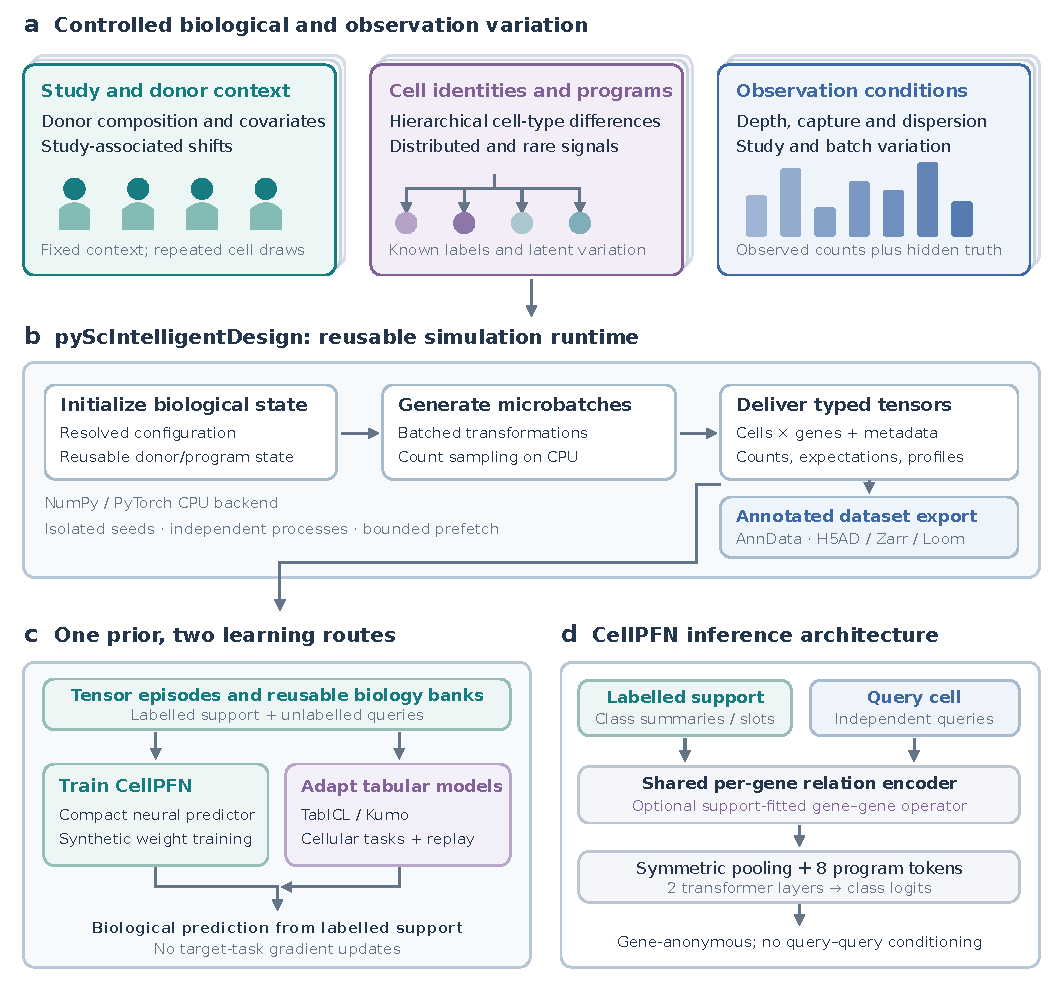
\includegraphics[width=\textwidth]{figures/architecture.pdf}
\caption{\textbf{A reusable cellular simulator supplies two learning routes.}
\textbf{a,} Configurable donor context, cell identities and expression programs are combined with observation conditions to generate cells with known labels and latent truth.
\textbf{b,} pyScIntelligentDesign separates initialization of biological state from repeated microbatch generation. CPU computation combines NumPy and PyTorch; typed tensors connect generation to training, while annotated exports support independent dataset use. Independent producer processes and bounded prefetch overlap task generation with training. Hidden profiles and expectations support diagnostics and are excluded from classifier inputs.
\textbf{c,} Tensor episodes and reusable biology banks train compact CellPFN or continue training released tabular models with cellular tasks and generic replay. Both applications perform downstream inference from labelled support without target-task gradient updates.
\textbf{d,} CellPFN compares each query with support-derived gene summaries and learned slots, optionally incorporating a support-fitted gene--gene operator. Symmetric aggregation and learned program tokens feed a transformer and class prediction head. The tokens are computational summaries, not annotated biological pathways. The schematic describes architecture and data flow; shapes do not represent measured quantities.}
\label{fig:architecture}
\end{figure}

\clearpage
\section*{Methods}
\subsection*{CellPFN prediction task and expression representations}
\label{methods:cellpfn-task}
An episode consists of a labelled support matrix $X_S\in\mathbb{R}_{\geq0}^{N\times G}$, support labels $y_S\in\{1,\ldots,C\}^{N}$ and a query matrix $X_Q\in\mathbb{R}_{\geq0}^{Q\times G}$. The same $G$ gene coordinates occur in support and query, but the network receives neither persistent gene identifiers nor donor, study or simulator metadata. Class names are localized to the support classes. CellPFN returns one logit for each query--class pair and class probabilities by softmax. Its parameters remain fixed during prediction; support fitting constructs episode-specific statistics and learned support summaries. Query cells share this support state but do not attend to one another. Consequently, changing the other query rows does not change a given row's prediction, apart from numerical effects of batching. The architecture is summarized in Fig.~\ref{fig:architecture} and Supplementary Table~\ref{tab:model-architecture}.

Count and processed-expression inputs use separate linear input projections and a shared nonlinear backbone. For count inputs, the delivered-panel depth is $d_i=\max(1,\sum_g x_{ig})$, the composition is $p_{ig}=x_{ig}/d_i$, and the expression view is $\ell_{ig}=\log(1+10^4p_{ig})$. Processed inputs must already contain nonnegative log-normalized expression; the supplied values are used as $\ell_{ig}$ without another normalization or logarithm. For either mode, we compute support-wide gene means $\bar\ell_g$, population standard deviations $s_g$ and detection fractions, together with the corresponding statistics within each support class. We use $\epsilon=10^{-6}$ and define the support-standardized view
\begin{equation}
 z_{ig}=\operatorname{clip}\!\left(\frac{\ell_{ig}-\bar\ell_g}{\max(s_g,\epsilon)},-8,8\right).
 \label{eq:model-standardization}
\end{equation}
The support statistics also transform query rows. This standardized log-expression view is an input feature, not a negative-binomial Pearson residual. Training assigns count and processed modes in a 70:30 mixture; processed training inputs are obtained by row-wise log-normalization over the complete delivered gene panel.


\subsection*{Cellular task prior and simulator architecture}
\label{sec:simulator}

pyScIntelligentDesign separates the definition of a synthetic experiment from the production of individual cells. A configuration specifies a distribution over gene abundance, cell populations, donor attributes and observation processes. Instantiating this distribution fixes the biological parameters of one experiment; repeated sampling then produces cells sharing its population and donor structure. The resulting prior supplies both CellPFN training episodes and the cellular tasks used to adapt tabular models (Fig.~\ref{fig:architecture}). The implementation also exposes an independent simulation interface for annotated single-cell datasets. We describe the cellular prior used in the principal training endpoint below; the baseline prior is a comparison specification, and optional software capabilities are distinguished in Supplementary Table~\ref{tab:software-capabilities}.

Let $G$ denote the number of anonymous genes, $c_i$ the cell type, $d_i$ the donor, and $s_i$ and $b_i$ the study and batch of cell $i$. An experiment contains a positive baseline composition $\boldsymbol\pi$ with $\sum_g\pi_g=1$, cell-type programs, donor metadata and shared nuisance parameters. Gene identities are procedural indices. A single permutation is applied consistently to all cells in a delivered task; no correspondence to named real genes is required. The experiment hierarchy has four studies with one batch per study and 16 generated donors. Fixed training banks use eight donors, eight cell types and 8,192 genes; bank construction and the subsequent selection of task targets are separate operations.

\subsection*{Biological variation and gene programs}
\label{sec:simulator-biology}

The abundance distribution combines a lognormal body with a sparse high-abundance component, following the use of heterogeneous gene means and outliers in single-cell simulation\cite{zappia2017splatter}. It is normalized to a composition and constrained so that no gene exceeds 10\% of baseline mass. Three biological task families generate distinct relationships between expression and cell type: distributed mean programs, intermittently expressed markers superimposed on stable mean programs, and signed covariance programs. The bank schedule allocates these families in a 2:1:1 ratio. Biological parameters and technical randomness have separate seed namespaces, permitting controlled changes to observation conditions without redefining the underlying experiment.

For mean-program tasks, sparse gene loadings are combined into class-dependent shifts, with a hierarchy producing shared variation among related classes. For a normalized gene-weight vector $\boldsymbol w$, the implementation centres a shift $\boldsymbol v$ by $v_g-\sum_h w_hv_h$ and scales its weighted squared magnitude to the configured energy. Class shifts use $w_g\propto\pi_g^{1/2}$; their final values are smoothly bounded by $L\tanh(v_g/L)$, with $L=4.5$. A class template is proportional to $\pi_g\exp(v_{cg})$. A construction is admitted only if every class template has maximum gene share at most 0.35, with at most 16 construction attempts. These bounds apply to the class template, rather than imposing the same bound on every fully perturbed cell.

The marker family adds a class-specific sparse marker set. A Bernoulli draw controls whether the marker program is expressed in a cell, and a lognormal multiplier varies its amplitude. Marker and class shifts are combined before saturation, preserving the same class-shift ceiling. Hidden subtypes add within-class modes whose offsets are centred using their Dirichlet mixture weights. This permits multimodality without introducing an arbitrary unweighted class-mean shift. Optional trajectories vary position along class-centred program directions, with cell-specific position jitter; class-by-study and class-by-donor interactions provide domain-dependent changes in expression. Both trajectory and interaction blocks are independently enabled with probability 0.25 in the principal specification.

The covariance family isolates information carried by relationships between genes. Six sparse programs $V_{jg}$ are arranged in three pairs. For each pair, $u_j$ is a Rademacher variable and $e_j\in\{-1,1\}$ has expectation $\rho$; the private class code supplies a sign $a_{cj}\in\{-1,1\}$. The latent coordinates are $z_{2j-1}=u_j$ and $z_{2j}=a_{cj}u_je_j$, so their marginal means are zero and their paired correlations have class-dependent signs. The biological profile is
\begin{equation}
 p^{\mathrm{bio}}_{ig}\propto\pi_g\left(1+\sum_{j=1}^{6}z_{ij}V_{jg}\right).
 \label{eq:simulator-covariance}
\end{equation}
Program construction enforces positivity and weighted centring. Thus the class signal is placed in covariance at this biological layer; downstream nuisance transformations and count sampling remain part of the complete observation model.

Within-type cell state combines an independent residual with shared sparse programs and a weaker quality-associated direction. If $r_{ig}$ is the energy-normalized residual and $h_{ig}$ the centred structured state, the combined shift is
\begin{equation}
 u_{ig}=\sqrt{1-f}\,r_{ig}+\sqrt f\,\kappa h_{ig}-o_g.
 \label{eq:simulator-state}
\end{equation}
Here $f$ is the structured fraction, $\kappa$ is fixed once per experiment using a separate reference sample of 256 cells per class, and $o_g$ partially compensates the mean introduced by exponentiating structured variation. Program genes are sampled with probabilities proportional to baseline abundance raised to an experiment-specific power. Programs can be shared across classes or restricted to one class. Their activation probabilities vary by donor through a Gaussian donor-by-program logit shift. Fixing the normalization reference before cell production prevents the state scale from depending on the requested batch size or cell order.

Donor metadata are generated using the simulator's vine-copula machinery. Continuous latent metadata are transformed to their public measurement scales, including age and sex. Centred, standardized metadata act through sparse anonymous gene directions, normalized by baseline-weighted energy; configurable nonlinear kernels introduce additional shared gene responses. Selected-target and other-metadata contributions are retained separately and multiplied without renormalizing the combined effect. These metadata generate labels and expression jointly; task labels are not imposed independently on a completed expression matrix. The distinction between donor-disjoint phenotype tasks and closed-set donor-identity tasks is maintained during episode construction.

The donor aging component adapts stochastic perturbations in normalized log-count coordinates\cite{meyer2024stochasticaging}. A profile is placed at fixed reference depth 1,500, transformed by $q_g=\log(1+x_g)/\max_h\log(1+x_h)$, perturbed by an initial Gaussian increment and a sequence of clipped Gaussian increments, and transformed back. Chronological age maps from the fixed 5--110-year coordinate system to 0--105 steps; generated donor ages span 60--90 years. Initial and per-step standard deviations are 0.01 and 0.005, respectively, with a lognormal donor rate of mean one and log-standard deviation 0.2. Gene-specific rate mixtures and donor jitter vary susceptibility. A donor's entire clipped walk is prepared once as an equivalent offset and lower/upper clipping map, then reused for all its cells; this preserves the sequential clipping operation while amortizing the step loop. Before compositional renormalization, expression is bounded to $e^{-1}$--$e^1$ times the unaged input. The direct metadata age direction is disabled when the clock is active. Separate configured components add directional age shifts and age-dependent cell-noise scaling; the latter scales deviations around the expected log-state shift, preserving that log-state expectation rather than mean expression after exponentiation. Parameter distributions are given in Supplementary Table~\ref{tab:simulator-parameters}.

\subsection*{Observation model and calibration}
\label{sec:simulator-observation}

The biological profile, metadata/aging effects, cell state, donor effects and study/batch effects are combined in log-expression space and normalized:
\begin{equation}
 p_{ig}=\frac{p^{\mathrm{bio}}_{ig}\exp(\Delta_{ig})}
 {\sum_h p^{\mathrm{bio}}_{ih}\exp(\Delta_{ih})}.
 \label{eq:simulator-profile}
\end{equation}
Here $\Delta_{ig}$ comprises the enabled shifts, with the aging component inserted through the log-ratio of aged to unaged biology so that metadata are not applied twice. Library size has a log-additive study--batch--donor--cell hierarchy,
\begin{equation}
 \log L_i=\ell_0+\ell^{\mathrm{study}}_{s_i}
 +\ell^{\mathrm{batch}}_{b_i}+\ell^{\mathrm{donor}}_{d_i}
 +\epsilon_i+\delta_0,
 \label{eq:simulator-library}
\end{equation}
with experiment-specific scale multipliers and a lower library bound of 50. The normalized profile is converted to counts through a gamma--Poisson model:
\begin{equation}
 A_{ig}\sim\operatorname{Gamma}(\tilde k_{ig},1/\tilde k_{ig}),\qquad
 \lambda_{ig}=L_ip_{ig}A_{ig},\qquad
 X_{ig}\mid\lambda_{ig}\sim\operatorname{Poisson}(\lambda_{ig}).
 \label{eq:simulator-counts}
\end{equation}
The second gamma argument is scale, giving unit mean and variance $1/\tilde k_{ig}$. Conditional on $L_i$, $p_{ig}$ and $\tilde k_{ig}$, integrating the gamma draw yields mean $L_ip_{ig}$ and variance $L_ip_{ig}+(L_ip_{ig})^2/\tilde k_{ig}$. The terminal Poisson sampler is applied exactly once.

Dispersion follows the realized class template where a class-mean template exists, and otherwise the baseline profile. At nominal mean $m_{cg}$,
\begin{equation}
 k_{cg}=\operatorname{clip}\!\left[
 \frac{J_g}{\phi_0+a\max(m_{cg},m_0)^{-\alpha}},\;0.01,\;160\right],
 \label{eq:simulator-dispersion}
\end{equation}
where $J_g$ is lognormal gene jitter, $\phi_0=0.1$, $m_0=0.1$, $\alpha=1.2$, and $a$ is drawn log-uniformly from 0.05--2.0. For the enabled age-dependent noise multiplier $m_{ig}^{\mathrm{age}}$, the sampler uses the effective shape $\tilde k_{ig}=\operatorname{clip}[k_{c_i g}/(m_{ig}^{\mathrm{age}})^2,0.01,160]$; without this modifier, $\tilde k_{ig}=k_{c_i g}$. The fitted dispersion is an effective observed-variation model; it does not identify all real overdispersion as technical noise. The principal cellular prior has explicit observation dropout disabled. Study-specific detection and structural gene absence are available for their named prior ablations. The general simulator additionally supports composable observation effects, described separately in the supplement.

Real data inform the prior through aggregate calibration targets. The principal ranges were selected to cover bank-matched summaries from ROSMAP, ZEBRA, PBMC CITE-seq and kidney, rather than reproduce one panel's medians. These summaries concern depth, dispersion, donor variation, abundance concentration, marker structure and separability. The calibrated objects are scalar parameters and distributions; the generator does not load real donor expression profiles or named-gene templates into training banks. Nevertheless, calibration and repeatedly inspected development evaluations used the same real datasets that contribute to the reported evaluations. Synthetic-only model training therefore does not imply a development procedure independent of real data, and the realism comparison is a prior-predictive diagnostic rather than independent validation. Baseline-prior comparisons retain their own configuration and population definitions.

\subsection*{Tensor interfaces, streaming and software extensibility}
\label{sec:simulator-software}

The software exposes three coordinated interfaces: configurable experiment objects, PyTorch-compatible cell streams\cite{paszke2019pytorch}, and annotated dataset export. A donor-expression provider supplies cell types, gene identifiers and donor-conditioned expression; an external provider can be registered through a Python factory without changing the experiment orchestrator. Generic observation effects implement a tensor-valued forward operation and compose in an owned \texttt{EffectStack}; governed stacks validate their topology and terminal count sampler. The cellular-prior provider instead owns its complete observation process, preventing a second application of technical noise through the generic stack.

The common output contract distinguishes normalized expected profiles, realized pre-sampling intensities and observed counts. All are matrices with shape cells $\times$ genes; profiles and intensities use float32 and counts use int32. Their dimensions, non-negativity, integer range and profile normalization are checked at the interface. Public metadata, sampling groups and provenance accompany the tensors, while hidden biological state and training-only sidecars remain separately controlled. This contract prevents a normalized profile from being silently interpreted as observed UMI counts.

\texttt{CellStream} is a PyTorch \texttt{IterableDataset}. It first reserves cell coordinates and then materializes a microbatch; the generic path groups cells sharing an effect stack before applying tensor operations. The cellular-prior kernel combines NumPy computations\cite{harris2020numpy} with PyTorch tensor interfaces and returns CPU tensors. The current stream implementation uses CPU generation and requires \texttt{num\_workers=0} in a local PyTorch DataLoader. Process-global Python, NumPy and Torch random states are isolated, activated and restored for each simulator instance. Concurrent generation is provided by independently seeded processes, rather than cloning an active simulator into DataLoader workers.

CellPFN's task producer uses spawned CPU workers with bounded prefetch and deterministic result delivery. Fixed biology banks amortize experiment initialization across multiple support/query views, while prefetch permits CPU production to overlap model consumption. Counts are stored as uint16 only when all values are exactly representable, otherwise retaining int32; there is no count clipping to meet a storage width. Task receipts bind configurations, seeds, shapes and array contents. The model-neutral adaptation bank stores expression views and local labels before model-specific preprocessing, allowing the same cellular tasks to be consumed in different model environments.

For independent simulation use, collators convert streamed output to AnnData\cite{virshup2024anndata}, preserving count layers, cell/gene annotations and runtime provenance. Public-data and hidden-ground-truth loggers support H5AD, Zarr and Loom outputs. Dense and sparse observed-count exports are available, but the sparse path retains dense expected profiles and intensities. Working memory for direct generation scales with the microbatch's cell-by-gene arrays plus fixed biological state; exported datasets and prefetched banks add their own storage. Thus scalability depends on the selected output contract as well as the sampler. The supplement specifies these memory terms and provides a minimal usage example. Architecture alone is not interpreted as a measured speedup or a completed million-cell benchmark.

\subsection*{Support summaries and same-gene neural relations}
\label{methods:cellpfn-backbone}
The support encoder applies a shared multilayer perceptron independently to each cell--gene pair. Its features include expression, standardized expression and detection, support-wide and class-specific moments, and, for count inputs, square-root composition (full definitions below). The two input projections have widths $10\rightarrow64$ and $9\rightarrow64$ for count and processed inputs, respectively, followed by GELU, a $64\rightarrow64$ linear map and layer normalization. For a sequence of gene features $h_g$, both the support and relation encoders use the symmetric reduction
\begin{equation}
 \mathcal R(h)=\left[\frac1G\sum_g h_g,\;
 \sqrt{\frac1G\sum_g h_g^{\odot2}+\epsilon},\;
 \max_g h_g,\;\log\sum_g e^{h_g}-\log G\right],
 \label{eq:gene-reduction}
\end{equation}
with componentwise operations. This retains average, energy, extreme and smoothly aggregated responses while allowing arbitrary gene counts and permutations, in the spirit of set-based representations\citep{zaheer2017deepsets}. The resulting 256-dimensional support-row vector is projected to 448 dimensions, followed by three residual, pre-normalized multilayer perceptron blocks with hidden width 1,792.

Within class $c$, learned inducing queries assign weights to support rows. If $e_i$ is the row embedding and $\bar e_c$ its class mean, summary $k$ has weights
\begin{equation}
 a_{cki}=\operatorname{softmax}_{i:y_i=c}
 \left[\frac{\langle f_q(\bar e_c+q_k),f_k(e_i)\rangle}{\sqrt{448}}\right].
 \label{eq:class-summary}
\end{equation}
Here $f_q$ and $f_k$ are learned affine maps from 448 to 448 dimensions. The implementation allocates eight summary slots and activates $\min(n_c,4)$, where $n_c$ is class support size; inactive slots are masked. At one support cell per class, precisely one summary is active. Each summary is a weighted average of the per-gene support views, retaining the correspondence between a query gene and that same gene in the support.

For every query $q$, class $c$, summary $k$ and gene $g$, the relation input concatenates the query view, the weighted support view, their elementwise product and absolute difference, and additional support statistics and row-level covariates. It has 28 channels for counts or 22 for processed expression. Separate $28/22\rightarrow448$ projections feed a shared GELU--linear--layer-normalization network producing 224 relation channels. Applying equation~\ref{eq:gene-reduction} across genes yields an 896-dimensional vector for each query--class--summary combination. A linear projection, GELU and layer normalization map this vector to 448 dimensions, and a learned summary-role embedding is added.

Eight learned program queries cross-attend to the active summary tokens using eight attention heads. The attended output is added to the program queries and layer-normalized. A learned token specifying count or processed mode is prepended, and the resulting nine tokens pass through two pre-normalized transformer layers\citep{vaswani2017attention}, each with eight heads, width 448, feed-forward width 1,792, GELU and zero dropout. Mean and maximum pooling over the eight transformed program tokens, excluding the mode token, yields an 896-dimensional vector $h_{qc}$. The direct classifier is a $896\rightarrow448\rightarrow1$ multilayer perceptron with GELU, producing one unbounded neural logit per class. Its output contains no fixed analytic score or residual correction to an external classifier. Support-derived analytic quantities are input features only. The backbone without the gene--gene operator has 11,925,345 learned parameters.

\subsection*{Support-fitted gene--gene operator}
\label{methods:gene-operator}
The operator supplies joint gene information to the neural relation and classification paths. It estimates pooled within-class covariance from the support-standardized vectors in equation~\ref{eq:model-standardization}. Let $\mu_c$ be the class mean of these vectors, $r_i=z_i-\mu_{y_i}$, and $\nu=\sum_c\max(n_c-1,0)$. A gene is support-variable if its maximum and minimum standardized support values differ. All other genes are masked from the operator, including its distances and channels. On the $G_\ast$ support-variable genes, for $\nu>0$, define
\begin{equation}
 v_g=\frac1\nu\sum_i r_{ig}^2,\qquad
 D_g=v_g+0.01\,\frac1{\max(G_\ast,1)}\sum_{g'}v_{g'}.
 \label{eq:operator-diagonal}
\end{equation}
If the additive floor is at most $10^{-10}$, it is replaced by 1; if $\nu=0$, the diagonal is the identity. These safeguards keep completely constant or within-class constant support finite. Masked genes have zero inverse scale.

We diagonalize the support-row Gram matrix of $R D^{-1/2}/\sqrt\nu$ in float64. From its leading eigenvalues $\eta_j$ and eigenvectors, we recover orthonormal gene loadings $U$ in the diagonally standardized coordinates. The number of candidate components is at most $\min(32,\lfloor\nu/2\rfloor,N)$; retained spikes are $\lambda_j=\max(\eta_j-1,0)$, with zero-spike components discarded. The implied covariance is
\begin{equation}
 \widehat\Sigma=D^{1/2}\left(I+U\operatorname{diag}(\lambda)U^\mathsf{T}\right)D^{1/2}.
 \label{eq:operator-covariance}
\end{equation}
This pooled estimator has no per-class low-rank subspaces. It is fitted without gradients from support cells alone; no trainable covariance matrix or gene-identity embedding is introduced.

For query--class difference $d_{qc}=z_q-\mu_c$, put $a_{qc}=D^{-1/2}d_{qc}$ and $b_{qc}=U^\mathsf{T}a_{qc}$. The squared Mahalanobis distance and whitened difference are
\begin{align}
 M_{qc}&=\|a_{qc}\|^2-\sum_j\frac{\lambda_j}{1+\lambda_j}b_{qcj}^{2},\label{eq:operator-mahalanobis}\\
 w_{qc}&=\left[I-U\operatorname{diag}\!\left(1-(1+\lambda)^{-1/2}\right)U^\mathsf{T}\right]a_{qc}.
 \label{eq:operator-whitening}
\end{align}
Before clipping, $\|w_{qc}\|^2=M_{qc}$; computed distances are lower-bounded by zero to remove round-off artifacts. The gate
\begin{equation}
 \gamma_c=\begin{cases}(n_c-1)/(n_c+3),&n_c\geq2,\\0,&n_c\leq1\end{cases}
 \label{eq:operator-gate}
\end{equation}
sets the operator's contribution to exactly zero for one-shot classes. The gene channel is $\gamma_c\operatorname{clip}(w_{qcg},-8,8)/4$. A bias-free $1\rightarrow448$ projection adds this channel to the relation network's input projection, shared across summaries.

The second path provides class-comparative operator information to the classifier. With $\mathcal C_+=\{c:n_c\geq2\}$, define
\begin{align}
 t_{qc}&=\frac{M_{qc}-|\mathcal C_+|^{-1}\sum_{c'\in\mathcal C_+}M_{qc'}}{\sqrt{2\max(G_\ast,1)}},\\
 s_{qc}&=\operatorname{asinh}(t_{qc})-
 \frac{\sum_{c'}\gamma_{c'}\operatorname{asinh}(t_{qc'})}{\sum_{c'}\gamma_{c'}}.
 \label{eq:operator-centered}
\end{align}
Empty-set denominators are replaced by 1; all contributions then vanish through the gate. If $r$ is the retained pooled rank, the three inputs are $u_{qc}=(\gamma_cs_{qc},\gamma_cr/32,\gamma_c)$. A $3\rightarrow448\rightarrow896$ GELU multilayer perceptron $f$ modifies the classifier input as $h_{qc}+\gamma_cf(u_{qc})$. Thus both the scalar inputs and the head output are gated. The second centering in equation~\ref{eq:operator-centered} ensures $\sum_c\gamma_cs_{qc}=0$ even for unequal support sizes. The gene projection and the output layer of $f$ are initialized to zero, preserving the common parent model's predictions at initialization. These paths add 404,544 parameters, giving 12,329,889 parameters in total.

We distinguish three trained arms: no operator, diagonal operator and full operator. The diagonal arm uses equations~\ref{eq:operator-diagonal}--\ref{eq:operator-centered} with no low-rank correction, $\widehat\Sigma=D$, while retaining the full support fit's rank scalar $r/32$. Its neural dimensions, gate and initialization match the full arm. The no-operator arm omits both added neural paths. All three arms continue from the same no-operator parent with matched task schedules. Separately, operator-off and rank-zero interventions remove pathways or low-rank corrections during inference with trained parameters fixed. These interventions measure dependence of an existing predictor on its operator; they are not substitutes for training the corresponding ablation. One-shot gating likewise does not require independently trained arms to agree, because their shared backbone parameters can diverge during training.

\subsection*{Reusable simulated banks, task sampling and optimization}
\label{methods:model-training}
The trainer receives simulated counts from pyScIntelligentDesign through a deterministic bank interface. Each independently seeded bank contains eight donors, eight cell types and 256 cells per donor--type combination at 8,192 parent genes. Thirty-two episodes reuse each bank with separately sampled targets, cells, gene panels, gene orders and class-label permutations. Four banks are interleaved, with one episode per bank in each four-task optimizer opportunity. Reuse therefore increases task exposure without creating additional independent biological datasets. During cellular-prior bank construction, a row with fewer than twenty counts receives up to eight technical redraws at the same biological coordinates. The highest-count attempt is retained, stopping when the threshold is reached; any remaining zero-count row invalidates the bank.

Targets comprise binary donor metadata, four-category donor metadata, cell type and donor identity. Metadata targets use one query donor per label and other eligible donors as support, within one selected cell type. Cell-type targets use two query donors and six support donors. Donor-identity tasks use the same donor classes but disjoint support and query cells. They consequently train identification, not transfer of a phenotype to unseen donors. The first 32 cells of every donor--type combination are reserved for diagnostics. Support cells are sampled by cycling across eligible donors. Metadata values are assigned native binary labels or rank-based binary/four-category labels without splitting ties; incompatible target fields are replaced by other eligible fields, and a bank with no compatible target produces a recorded zero-weight task.

Support budgets are drawn from 1, 10 and 100 cells per class with probability 0.25 each, 2, 4, 8 and 16 with probability 0.04 each, and 32 and 64 with probability 0.045 each. Requested gene panels contain 2,048, 4,096 or 8,192 genes, sampled without replacement and permuted jointly for support and query. A 12.5-million-element cap reduces gene width when necessary while preserving requested cell counts. The nominal query budget is 100 cells per class; in the cellular prior's cell-type tasks, the total $100C$ is distributed according to available class frequencies. The curriculum laws, target allocation and admission rules are specified in Supplementary Table~\ref{tab:training-recipe}.

The evaluated model was trained on 320,000 scheduled episodes from 10,000 baseline-prior banks, followed by 64,000 episodes from 2,000 banks of the cellular prior. The gene--gene paths were added at the start of this 64,000-episode stage. There were 96,000 optimizer opportunities in total; 276,828 episodes contributed nonzero loss, including all 64,000 final-stage episodes. These are distinct from the number of banks or simulated cells. All CellPFN arms use model seed 42 and task-stream seed 15113. The endpoint was the declared training milestone, rather than a checkpoint selected by maximum real-panel accuracy. Real summaries informed simulator calibration, and development panels informed design decisions; synthetic-only optimization does not imply that the complete research process was independent of real data.

The objective is mean query cross-entropy within each task, averaged uniformly over accepted tasks in an optimizer opportunity. Rejected tasks contribute zero weight; an opportunity with no accepted task does not apply an optimizer step. AdamW\citep{loshchilov2019adamw} uses $\beta_1=0.9$, $\beta_2=0.999$ and weight decay $10^{-4}$. Its learning-rate multiplier has 8,000 warm-up opportunities and cosine decay to a 0.1 floor over a 200,000-opportunity horizon. The base rate is $10^{-4}$ for the first 40,000 opportunities and $10^{-5}$ thereafter. At the operator stage, pre-existing Adam moments and counters are restored by parameter name; new operator parameters start with fresh optimizer state and use ten times the backbone rate, multiplied by a linear 1,000-opportunity ramp. Backbone and operator parameter groups are separately clipped to gradient norm 5. Training uses PyTorch\citep{paszke2019pytorch} with bfloat16 autocast on NVIDIA H100 80-GB GPUs; feature statistics and losses use float32 and the covariance fit uses float64. Gene and query--class chunking, and activation checkpointing during training, bound working memory without changing the mathematical reduction.

\subsection*{Continued training of tabular foundation models}
\label{methods:tabular-adaptation}
We initialized TabICL and the small and large Kumo Tabular models from their released weights\citep{qu2026tabiclv2,nvidia2026kumo}. The three adaptation arms consumed the same cellular task stream and generic replay tables. Each of 2,500 updates contained 16 cellular tasks and four generic tables: 40,000 cellular tasks and 10,000 replay tasks. Cellular tasks retained the simulator's target construction, used 1, 10 or 100 support cells per class in exact thirds over consecutive triples of tasks, and used 32 query cells per class. Task families followed the final curriculum probabilities (60\% binary metadata, 20\% categorical metadata, 15\% cell type and 5\% donor identity), with no more than eight classes.

Cellular counts were log-normalized and transformed using support-fitted 2k HVGs or a principal-component view with at most 100 components. View choice, preprocessing ensemble choice and randomness were recorded per task. Neither feature selection, standardization nor projection was fitted to query rows. TabICL used its support-fitted ensemble generator, with identity or power normalization, Latin feature shuffling, shifted class labels and outlier threshold 4. Training used one or two ensemble members per cellular task, averaging their query cross-entropies. Kumo used its own default preprocessing recipe fitted to support rows: four recipe members expose its four numerical transformations, and the task plan selects one or two members for gradient accumulation. Gradients pass through the classifier behind Kumo's class-count wrapper. The module remains in evaluation mode during this differentiable route, which has no dropout or batch-statistic update.

Generic replay tables were drawn from TabICL's mixed structural-causal-model prior with 5--100 features, at most ten classes, at most 1,024 rows and support fractions between 0.1 and 0.9. For Kumo, replay query rows whose class is absent from support are masked. The update loss averages valid task losses. All three principal adaptation arms used float32 training, AdamW with peak learning rate $3\times10^{-5}$, zero weight decay, $\beta=(0.9,0.999)$, 125 linear warm-up updates, cosine decay to zero at update 2,500 and global norm clipping at 1. Recorded invalid tasks were bounded by a cap of 40, rather than silently replaced. Checkpoints at updates 313, 625, 1,250 and 2,500 correspond to approximately 5,000 and exactly 10,000, 20,000 and 40,000 cellular tasks. Evaluation used each model's deployment preprocessing; Kumo used eight ensemble members for the small model and 16 for the large model, with seed 0. No additional supervised head was fitted for these in-context predictions.

The generic-only Kumo control replaced the 16 cellular slots with generic tables and retained four replay slots; its row and column counts were not matched to the cellular stream. Two further cellular task draws retained the same released initialization and model seed, quantifying task-sampling variation rather than independent initialization variation. Prior-content proxy comparisons used the same adaptation machinery and a declared 10,000-cellular-task endpoint on the 2,500-update schedule. Changes in task family, donor count or class composition are reported as interventions in that distribution, not architectural changes.

\subsection*{Biological datasets and support--query separation}

PBMC evaluation used the 3-prime RNA component of the Hao et al. CITE-seq reference\cite{hao2021multimodal}: GEO accession GSE164378, RNA sample GSM5008737 and the supplied cell metadata. The source contains 161,764 cells and 33,538 RNA coordinates. Published annotations combine RNA, measured surface proteins and curation; they are not an independent protein-only ground truth. Predictions used RNA alone. Barcodes joined the original RNA matrix to metadata, and RNA library sums were checked against the metadata. The accompanying antibody measurements and annotations were audited against the author-linked reproduction snapshot; antibody measurements were not prediction inputs. Cells annotated as doublets were excluded. A class was eligible only when it contained at least 25 cells in each support donor and ten in each query donor, yielding eight broad and twenty finer classes.

Support donors were P1, P3, P5 and P7; query donors were P2, P4, P6 and P8. All timepoints of a donor remained on the same side, with two donors from each acquisition batch on each side. Ten query cells per class and donor were selected by deterministic metadata-based SHA256 rankings, giving 320 and 800 query cells for the broad and fine tasks. Within each class and support draw, donor and cell rankings were shuffled deterministically and sampled round-robin across donors. Prefixes supplied one, ten or 100 support cells per class; at 100 supports, each donor contributed 25 cells. Query cells were fixed across support budgets, draws and methods. The primary comparison used support draws 0--2; extended diagnostics followed the same sampling rule with more draws.

Human cortex evaluation used the 50,000-cell ZEBRA benchmark subsample\cite{flotho2024zebra}, with 21,158 genes and four broad classes: glia, immune, neural and vascular cells. The shared support pool comprised Bakken, Gerrits, Nagy, Schirmer, Trobisch and Yang Cortex studies. Development queries comprised 7,769 cells from 59 recorded donors in Absinta, Kihara, Lim and Velmeshev studies; held-out-study queries comprised 7,163 cells from 34 recorded donors in Hardwick, Herring, Jaekel and Yang studies. Support and query studies were disjoint, and query cells remained fixed across budgets and methods. Both query panels nevertheless contributed to model development; the held-out-study designation describes their study separation, not an untouched final model-selection set. Frozen cell identifiers, study assignments and input-file hashes define these panels more precisely than publication names alone.

The secondary kidney evaluation used healthy living-donor data from GSE202109\cite{mcevoy2022kidney}, distributed through CELLxGENE, with 27,675 cells from 19 donors and 26,791 measured genes. Three donor-held-out folds evaluated five- and nine-class cell-type tasks and proximal-tubule sex prediction. Cell-type tasks supplied 100 supports per class and 40 query cells per class. Sex prediction used six or seven query donors per fold, with five query cells per donor. Two 4,096-gene panels were retained: a kidney-support-derived panel and a panel derived from the historical ZEBRA support pool. These feature panels therefore used more support information than an individual few-shot case. Kidney cell-type accuracy and donor-level sex accuracy were kept separate.

\subsection*{Expression inputs and feature selection}

CellPFN received original counts for PBMC and the supplied processed expression for the primary cortex analysis. Count-based comparator inputs were transformed to $\log[1+10^4x_{ig}/\sum_hx_{ih}]$, using each cell's full measured library before gene selection. Supplied ZEBRA log-transformed counts per 10,000 were passed through unchanged. Genes unavailable in individual ZEBRA studies had been stored as zeros; this preprocessing artifact was evaluated separately from biological non-expression.

Highly variable genes were selected using labelled support rows only. The implementation exponentiated log-expression, computed gene means and unbiased variances, and standardized log dispersion within 20 mean-expression bins, following the Seurat-flavour dispersion statistic. Finite scores were ranked with a deterministic tie break based on the anonymous support column, retaining at most 2,000 or 8,192 genes. The same selected columns and order were applied to queries. Table labels denote requested HVG caps. In the three primary one-shot draws, the 8,192-HVG view retained 6,995--7,647 genes for broad PBMC and 2,209--5,301 for cortex; finite support variation could therefore reduce the realized width below the requested cap. Principal-component controls standardized support-selected genes, clipped standardized values to $[-10,10]$, fitted the decomposition to support rows, and retained $\min(100,n_{\mathrm{support}}-1,n_{\mathrm{genes}})$ components. Query expression did not influence selection, scaling or projection.

The cortex sensitivity analysis reconstructed integer counts from the lattice of the supplied processed values and retained 12,325 genes measured across eligible contributing studies. Reconstruction was conditional on the smallest positive expression level representing one count, rather than a retrieval of original sequencing counts. A matched processed partner was recomputed from the reconstructed common panel. Query identities and labels were unchanged; some supports changed after reconstruction-ineligible cells were removed. Consequently, historical full-panel and common-panel results do not isolate count versus processed representation. The reconstruction rule and support replacement are specified in the technical supplement.

\subsection*{Comparator models and selection}

Released tabular comparators were TabICLv2, TabPFN-3.5 and Kumo Tabular small and large\cite{qu2026tabiclv2,jaeger2026tabpfn35,nvidia2026kumo}. Each used labelled support cells as context, with no target-task gradient update. Continued-training checkpoints used the same inference route as their released reference. Main comparisons used support-selected 2,000-gene inputs; scaling analyses separately evaluated 8,192-gene and all-gene inputs. Package-default transformations, feature subsampling and feature limits remained active. Refused inputs and unevaluated cases were recorded as missing, not as zero accuracy. TabPFN-3.5 results were obtained under its non-commercial research terms\cite{priorlabs2026tabpfn35card}.

Geneformer-V2-316M\cite{chen2026geneformer} and the whole-human scGPT checkpoint\cite{cui2024scgpt} supplied frozen embeddings. Geneformer used Ensembl-linked rank-value tokens and mean embeddings; scGPT used gene-symbol inputs, binned values and unit-length CLS embeddings. Logistic classifiers were fitted to support embeddings only. Geneformer used support-standardized embeddings; scGPT used unscaled embeddings. Exact token limits, classifier settings and recorded software releases are listed in Table~\ref{tab:evaluation-settings}. Native input routes were preserved, so these comparisons jointly reflect representation, feature coverage and classifier choice.

Support-trained comparators included nearest-class-mean and prototype rules, logistic regression, diagonal and low-rank LDA, CellTypist\cite{dominguezconde2022celltypist}, SingleR\cite{aran2019singler} and scANVI\cite{xu2021scanvi}. CellTypist was fitted to the selected supports without query majority voting. SingleR used the supports as its reference. Inductive scANVI used supports only; its separately labelled transductive comparison also used unlabelled query cells and a donor batch key. Processed cortex inputs were not passed to count-likelihood scANVI. LDA diagnostic rows were available at ten and 100 supports, not one support per class. The inductive scANVI recipe used batch size 128, a 90\% training fraction and ten supervised epochs without class-balanced replacement sampling. At fine-PBMC one-shot support, 18 of 20 labelled cells entered optimization, leaving at least two classes without a training example. These low-support results describe that fixed recipe. SingleR retained its default classic marker mode rather than the alternative recommended for single-cell references.

The displayed family representatives were chosen within the development evaluation. Kumo size selection used the mean across the twelve core panel--budget combinations on 2,000 genes; the CellPFN reference was an explicitly selected model state, and logistic heads were the declared primary heads for Geneformer and scGPT. These choices were not independently validated model-selection procedures. Study-level pretraining overlap was assessed separately from benchmark support--query separation, using the recorded corpus/source-study audit. Such matches indicate possible unlabelled query-source exposure; they do not establish identical cell inclusion, target-label exposure or supervised leakage.

\subsection*{Exploratory subtype and sex tasks}

The eight PBMC subtype tasks comprised level-2 CD4 and combined T-cell siblings, level-3 CD4, CD8, B, NK and combined T-cell siblings, and the complete eligible level-3 vocabulary. They inherited the PBMC donor split and class-availability rules. Candidate selection was conducted after the prior-ablation read-outs and is exploratory. It used nearest-class-mean and logistic-reference performance, not CellPFN or proxy predictions: at 100 supports, the larger reference accuracy had to reach a chance-corrected skill of 0.20 while remaining below 85\% balanced accuracy. Each task used ten support draws at one and ten supports and five draws at 100 supports. CellPFN received up to 8,192 support-selected genes; the Kumo-small proxy received up to 2,000. Supplied CellPFN task means were reported without constructing intervals from unavailable individual-case predictions. Two exploratory cortex tasks used the same reference checkpoint and up to 8,192 HVGs: seven development labels and three held-study neural labels, defined in Supplementary Table~\ref{tab:s9}. They used ten, ten and five support draws at one, ten and 100 supports; the supplied checkpoint means do not include draw-level uncertainty. Changes in labels and evaluated cells preclude interpreting their difference from the primary broad-class benchmark as an isolated difficulty effect.

The original ZEBRA sex task used Sayed oligodendrocytes, 100 support cells per sex from twelve GSM samples, and 50 query cells from ten other GSM samples. GSM separation was not interpreted as independently verified donor separation. Later study-matched sex tasks used ten splits, four to 32 support units per sex, ten cells per support unit and twenty per query unit. The positive control required measurement of XIST and at least four specified Y-linked genes; a broader task included additional studies with a different common gene universe. Units were persons except for age-by-sex groups of GSM samples in Sayed. Reused persons and unresolved cross-study identity overlap preclude treating the ten splits as independent cohorts. Scores were averaged within query units before unit-level AUC calculation. \unresolvedclaim{O06}{Gene-level attribution for these sex tasks remains unavailable; eligibility based on sex-linked genes does not demonstrate that those genes drove the model's predictions.}

\subsection*{Metrics and uncertainty}

Balanced accuracy was the mean recall across every declared query class. Negative log-likelihood was the mean negative log probability of the true class, in nats; expected calibration error used fifteen fixed-width confidence bins. Probabilities and class order were checked before scoring. Performance means first averaged support draws within a panel--budget combination and then weighted the twelve combinations equally. Low-support summaries averaged the eight combinations with one or ten supports. Paired comparisons matched model, panel, input view, support budget and draw; a difference between unmatched views was not interpreted as an isolated model effect.

Three-draw benchmarks are descriptive and use ranges or individual values. The ten- and twenty-draw diagnostics used Student $t$ intervals over support draws, paired for contrasts. These quantify sensitivity to labelled-context sampling conditional on the chosen cohorts and weights. Every trained arm had one model seed; task-stream replicates did not estimate variation across independently initialized models. Kidney fold differences combine cohort and support variation. The nested PBMC subtype tasks share cells and labels and are not independent biological replicates. Attribution case ranges and single-run timings were not assigned confidence intervals. Missing, refused and unrun values were never replaced by zero.

\subsection*{Query-gene deletion and attribution validation}

For a query $x$ and fixed support set $S$, let $a$ and $b$ be the initially highest- and second-highest-logit classes. Define the fixed-pair margin $m(x;S)=f_a(x;S)-f_b(x;S)$. The exact deletion target for gene $g$ was
\begin{equation}
 I_g(x;S)=m(x;S)-m(x^{(g\leftarrow0)};S).
\end{equation}
Only the query gene was set to zero; support summaries and the fitted covariance operator were held fixed. A positive effect supports the original predicted class relative to its original runner-up. It is neither an expression-direction statistic nor an experimental perturbation effect. Negative effects oppose this fixed-pair margin. A gene already at zero has zero deletion effect, so this intervention cannot measure predictive information carried by its absence.

DS-LOO updates the mean, root-mean-square, maximum and log-sum-exp pools when each per-gene relation vector is replaced by its zero-expression counterpart. A first-order expansion through the prediction head maps these pooled changes to margin changes. An additional gradient calculation corrects the read-depth coupling in count mode and the detected-gene fraction. This is an attribution sweep with head differentiation and corrections, rather than one ordinary prediction or exact model evaluation per gene. The supported mathematical approximation is detailed in the technical supplement. \unresolvedclaim{M01}{The production attribution implementation, exact normalization corrections and treatment of query-side operator coupling remain to be reconciled with the recorded analysis before the procedure is fully reproducible.}

Validation used six case configurations and both the reference and no-operator model: three PBMC cases, one cortex case, and one kidney case evaluated in count and processed modes. Cells had to be correctly classified under both stored bfloat16 predictions and the float32 rerun. Seeded sampling selected at most 24 cells per class, or 40 for kidney. Exact deletion was evaluated on unions of method-selected genes and random expressed genes, with additional DS-LOO extreme-ranked genes; it was not exhaustive over all genes. Rank correlations were computed within cells, then summarized by the recorded class/case aggregation; relative Euclidean error compared estimated and exact effect vectors. Deletion curves recomputed the fixed-pair margin after removing sets of ranked query genes. Gene symbols were restored after prediction for descriptive marker comparisons. No marker enrichment test was performed. Timings distinguished measured attribution runs from extrapolated exhaustive-deletion costs; comparisons made under shared GPU load remain provisional.

\subsection*{Provisional neuropathology analysis}

\unresolvedclaim{O02}{The ROSMAP analysis used aggregate records for donor-disjoint splits of neuropathology contrasts\cite{bennett2018rosmap}: CERAD 4 versus 1, CERAD 3--4 versus 1--2, and Braak 0--II versus V--VI. Support and query allocation was matched within sex on source and age bin. Each support donor contributed eighteen cells and each query donor twenty. Donor-level AUC was summarized over ten overlapping random splits using the reported corrected repeated-split interval. The exact sequencing-release crosswalk, donor-label corrections and CellPFN input-mode record remain unresolved, and these analyses must be rerun after cohort definitions are frozen.}

\clearpage
\nolinenumbers
\bibliographystyle{unsrtnat}
\bibliography{references}
\clearpage
\clearpage
\section*{Supporting quantitative results}
\begingroup
\setstretch{1.0}
\small
\setlength{\tabcolsep}{3pt}
\setlength{\LTpre}{8pt}
\setlength{\LTpost}{8pt}
\setcounter{table}{0}
\renewcommand{\thetable}{S\arabic{table}}
\renewcommand{\theHtable}{supp.\arabic{table}}
These tables accompany the main Results and retain negative findings, exploratory analyses and limits on replication. Unless stated otherwise, intervals describe variation over support draws for fixed models and query panels; they do not represent independent model training or population-level biological replication.
\begin{longtable}{@{}>{\raggedright\arraybackslash}p{4.5cm}>{\raggedright\arraybackslash}p{3.45cm}>{\raggedright\arraybackslash}p{3.45cm}>{\raggedright\arraybackslash}p{3.45cm}@{}}
\caption{Panel-specific benchmark performance and contextual baselines.}\label{tab:s1}\\
\toprule
Model & 1 support/class & 10 supports/class & 100 supports/class \\
\midrule\endfirsthead
\multicolumn{4}{l}{\small Table \thetable{} (continued)}\\\toprule
Model & 1 support/class & 10 supports/class & 100 supports/class \\
\midrule\endhead
\bottomrule\endfoot
\multicolumn{4}{@{}l}{\textbf{PBMC coarse}}\\
CellPFN & 60.1 [52.5, 70.9] & 84.0 [81.9, 85.9] & 91.9 [91.6, 92.2] \\
TabICLv2 & 50.2 [41.3, 58.4] & 81.4 [79.4, 83.1] & 92.4 [91.3, 93.4] \\
TabICLv2 + cellular prior & 62.3 [48.1, 72.5] & \textbf{85.2} [81.9, 88.1] & \textbf{93.4} [93.1, 94.1] \\
Kumo small & 45.8 [40.3, 50.3] & 82.2 [80.6, 83.4] & 92.6 [91.6, 94.7] \\
Kumo small + cellular prior & \textbf{62.8} [52.8, 69.7] & 83.3 [80.9, 86.3] & 92.3 [91.6, 93.1] \\
Kumo large & 58.9 [46.3, 65.6] & 81.7 [78.8, 83.8] & 92.8 [91.9, 93.8] \\
Kumo large + cellular prior & 62.2 [50.3, 70.0] & 82.5 [79.4, 85.0] & 92.8 [91.9, 93.4] \\
TabPFN-3.5 & 34.3 [30.9, 38.4] & 82.6 [80.6, 83.8] & 91.5 [90.0, 92.5] \\
Geneformer-V2 + LR & \textcolor{black!55}{\textbf{67.1}\textsuperscript{*} [58.1, 74.7]} & \textcolor{black!55}{\textbf{88.5}\textsuperscript{*} [86.9, 90.3]} & \textcolor{black!55}{92.7\textsuperscript{*} [91.6, 93.4]} \\
scGPT + LR & \textcolor{black!55}{64.9\textsuperscript{*} [53.1, 72.2]} & \textcolor{black!55}{77.5\textsuperscript{*} [75.6, 78.8]} & \textcolor{black!55}{80.7\textsuperscript{*} [80.3, 81.3]} \\
Low-rank LDA & -- & 79.4 [78.8, 80.0] & 90.0 [89.7, 90.3] \\
CellTypist & 39.8 [33.8, 47.5] & 77.5 [76.9, 78.1] & 87.8 [87.5, 88.1] \\
SingleR & 56.7 [52.8, 60.9] & 78.2 [74.1, 80.9] & 85.9 [85.0, 86.6] \\
scANVI inductive & 20.0 [11.3, 32.5] & 40.7 [26.6, 51.3] & 86.7 [86.6, 86.9] \\
scANVI transductive & 40.5 [36.3, 44.1] & 69.1 [65.9, 74.7] & 89.1 [88.1, 90.9] \\
Logistic regression & 37.5 [34.4, 43.4] & 80.5 [79.1, 81.6] & 91.7 [90.6, 93.1] \\
\addlinespace
\multicolumn{4}{@{}l}{\textbf{PBMC fine}}\\
CellPFN & \textbf{51.1} [44.8, 55.4] & 79.0 [77.6, 80.4] & 89.0 [88.6, 89.1] \\
TabICLv2 & 30.0 [26.8, 34.3] & 73.8 [72.1, 75.6] & 83.6 [82.9, 84.5] \\
TabICLv2 + cellular prior & 29.1 [26.4, 32.3] & 64.6 [61.0, 67.9] & 85.3 [84.3, 86.1] \\
Kumo small & 44.1 [43.6, 44.6] & 80.0 [79.4, 80.4] & 88.3 [88.1, 88.4] \\
Kumo small + cellular prior & 49.0 [45.9, 52.3] & 80.5 [80.0, 81.0] & 88.7 [87.6, 89.6] \\
Kumo large & 46.3 [42.3, 50.0] & \textbf{83.3} [82.8, 83.6] & \textbf{89.3} [89.1, 89.5] \\
Kumo large + cellular prior & 50.9 [47.0, 55.8] & 82.2 [81.4, 83.5] & 89.2 [89.1, 89.4] \\
TabPFN-3.5 & 33.0 [29.4, 36.5] & 79.3 [77.4, 80.4] & 86.9 [86.5, 87.3] \\
Geneformer-V2 + LR & \textcolor{black!55}{\textbf{68.8}\textsuperscript{*} [66.6, 70.9]} & \textcolor{black!55}{\textbf{84.9}\textsuperscript{*} [84.3, 85.5]} & \textcolor{black!55}{\textbf{90.4}\textsuperscript{*} [90.0, 90.9]} \\
scGPT + LR & \textcolor{black!55}{55.7\textsuperscript{*} [51.3, 58.1]} & \textcolor{black!55}{65.9\textsuperscript{*} [65.3, 67.1]} & \textcolor{black!55}{72.0\textsuperscript{*} [71.5, 72.9]} \\
Low-rank LDA & -- & 70.3 [70.0, 70.5] & 87.8 [87.5, 87.9] \\
CellTypist & 33.9 [26.8, 37.8] & 69.7 [68.6, 70.8] & 84.2 [83.9, 84.6] \\
SingleR & 46.0 [42.1, 51.8] & 68.6 [67.0, 70.1] & 83.3 [82.6, 83.9] \\
scANVI inductive & 21.7 [14.4, 26.1] & 51.8 [50.8, 53.4] & 83.9 [81.6, 85.3] \\
scANVI transductive & 40.8 [39.5, 41.5] & 70.8 [68.8, 74.0] & 86.2 [85.8, 86.5] \\
Logistic regression & 39.0 [34.0, 46.8] & 73.4 [71.8, 75.9] & 85.1 [84.4, 85.6] \\
\addlinespace
\multicolumn{4}{@{}l}{\textbf{ZEBRA development}}\\
CellPFN & 41.4 [33.1, 47.4] & \textbf{63.6} [61.9, 65.6] & \textbf{66.1} [65.8, 66.4] \\
TabICLv2 & 39.5 [33.4, 42.6] & 59.9 [57.9, 62.2] & 65.3 [64.9, 65.7] \\
TabICLv2 + cellular prior & 44.6 [35.9, 57.1] & 60.6 [57.4, 62.6] & 65.3 [65.1, 65.5] \\
Kumo small & 31.2 [26.6, 36.4] & 57.5 [50.5, 61.7] & 65.1 [64.5, 65.7] \\
Kumo small + cellular prior & 41.9 [34.9, 51.2] & 59.2 [53.4, 62.3] & 64.9 [63.8, 65.6] \\
Kumo large & 40.1 [38.2, 41.5] & 56.8 [49.2, 61.2] & 65.1 [64.9, 65.3] \\
Kumo large + cellular prior & 42.8 [37.3, 52.3] & 60.6 [55.6, 63.4] & 65.8 [65.6, 66.1] \\
TabPFN-3.5 & 38.4 [32.8, 43.3] & 59.3 [56.6, 60.8] & 65.5 [64.8, 66.0] \\
Geneformer-V2 + LR & \textcolor{black!55}{43.1\textsuperscript{(*)} [34.8, 50.2]} & \textcolor{black!55}{61.1\textsuperscript{(*)} [55.3, 66.7]} & \textcolor{black!55}{65.4\textsuperscript{(*)} [65.3, 65.5]} \\
scGPT + LR & \textbf{47.6} [43.7, 55.0] & 60.2 [53.2, 66.5] & 65.8 [65.6, 66.1] \\
Low-rank LDA & -- & 60.6 [58.4, 62.0] & 66.0 [65.8, 66.4] \\
CellTypist & 34.9 [32.6, 37.3] & 57.8 [48.6, 64.0] & 63.9 [63.5, 64.6] \\
SingleR & 44.4 [34.4, 53.3] & 61.7 [59.8, 63.5] & 63.9 [63.2, 64.2] \\
scANVI inductive & -- & -- & -- \\
scANVI transductive & -- & -- & -- \\
Logistic regression & 34.7 [28.1, 39.6] & 57.4 [48.7, 62.4] & 65.5 [65.1, 65.8] \\
\addlinespace
\multicolumn{4}{@{}l}{\textbf{ZEBRA held-study}}\\
CellPFN & 62.8 [45.2, 77.1] & \textbf{91.9} [88.6, 94.7] & \textbf{94.7} [94.3, 95.0] \\
TabICLv2 & 49.8 [46.6, 55.2] & 83.2 [75.5, 88.1] & 92.9 [92.1, 93.5] \\
TabICLv2 + cellular prior & 62.7 [37.8, 81.0] & 85.8 [81.9, 88.7] & 93.2 [92.2, 94.0] \\
Kumo small & 48.8 [31.7, 65.9] & 84.8 [81.3, 86.7] & 93.7 [92.3, 94.7] \\
Kumo small + cellular prior & 59.3 [41.8, 73.5] & 86.8 [83.4, 88.7] & 92.9 [91.1, 94.4] \\
Kumo large & 49.1 [39.6, 56.6] & 85.1 [80.3, 88.8] & 93.1 [91.7, 94.5] \\
Kumo large + cellular prior & 60.8 [39.1, 75.8] & 85.9 [81.4, 88.6] & 93.4 [93.2, 93.6] \\
TabPFN-3.5 & 54.1 [48.0, 65.3] & 85.3 [84.9, 85.8] & 93.9 [92.5, 95.3] \\
Geneformer-V2 + LR & \textcolor{black!55}{58.4\textsuperscript{*} [44.2, 72.5]} & \textcolor{black!55}{87.4\textsuperscript{*} [83.8, 91.7]} & \textcolor{black!55}{90.3\textsuperscript{*} [88.4, 92.6]} \\
scGPT + LR & \textbf{65.5} [52.5, 80.7] & 87.2 [80.6, 93.1] & 89.5 [88.9, 90.2] \\
Low-rank LDA & -- & 91.0 [89.6, 93.8] & \textbf{94.7} [94.0, 95.4] \\
CellTypist & 44.4 [41.6, 47.5] & 87.8 [80.4, 92.5] & 91.4 [90.6, 92.3] \\
SingleR & 56.8 [38.4, 71.1] & 86.6 [79.7, 90.8] & 89.1 [86.8, 90.6] \\
scANVI inductive & -- & -- & -- \\
scANVI transductive & -- & -- & -- \\
Logistic regression & 45.0 [42.1, 48.1] & 73.5 [70.7, 76.0] & 90.6 [90.0, 91.5] \\
\addlinespace
\end{longtable}
Values are mean [minimum, maximum] balanced accuracy (\%) over the same three support draws, not confidence intervals. Within each panel and support budget, bold identifies the highest mean overall and among unflagged comparators, including ties at displayed precision. Gray means and ranges carry the exposure stars defined in Table~\ref{table:overview}; unflagged entries do not certify absence of exposure. Inputs follow Table~\ref{table:overview}; CellTypist, SingleR and low-rank LDA use all genes, whereas logistic regression and scANVI use 2k HVGs. CellTypist\citep{dominguezconde2022celltypist} is fitted to the support cells; SingleR\citep{aran2019singler} uses the declared reference route. The scANVI\citep{xu2021scanvi} transductive route additionally uses the unlabelled query pool and is contextual rather than an inductive comparison. Dashes are missing evaluations, never zero accuracy. All selected fitted model checkpoints have one training seed; support-draw variation does not measure training uncertainty. Geneformer-V2 uses the 316M checkpoint. Source-study corpus overlap does not establish exact-cell or target-label exposure. Native gene vocabularies and training histories differ. Family variants were selected in the export and the evaluation is not a newly frozen independent benchmark.

\clearpage
\begin{longtable}{@{}>{\raggedright\arraybackslash}p{4.4cm}>{\raggedright\arraybackslash}p{6.5cm}>{\raggedright\arraybackslash}p{3.95cm}@{}}
\caption{Training exposure, prior transfer and generic-task retention.}\label{tab:s2}\\
\toprule
Model & Quantity & Count \\
\midrule\endfirsthead
\multicolumn{3}{l}{\small Table \thetable{} (continued)}\\\toprule
Model & Quantity & Count \\
\midrule\endhead
\bottomrule\endfoot
CellPFN & Parameters & 12329889 \\
CellPFN & Optimizer updates & 96000 \\
CellPFN & Simulated banks & 12000 \\
CellPFN & Scheduled episodes & 384000 \\
CellPFN & Loss-bearing episodes & 276828 \\
TabICLv2 & Parameters & 27552258 \\
TabICLv2 & Additional cellular tasks & 40000 \\
TabICLv2 & Adaptation updates & 2500 \\
Kumo small & Parameters & 27458266 \\
Kumo small & Additional cellular tasks & 40000 \\
Kumo small & Adaptation updates & 2500 \\
Kumo large & Parameters & 213668250 \\
Kumo large & Additional cellular tasks & 40000 \\
Kumo large & Adaptation updates & 2500 \\
\end{longtable}
CellPFN banks are reused for multiple episodes; scheduled and loss-bearing episodes are distinct. Adaptation uses 40,000 cellular tasks and 10,000 generic replay tasks per arm. Released-model pretraining precedes this adaptation and is not included in these counts. TabICLv2 reports 35 million synthetic pretraining datasets\citep{qu2026tabiclv2}; this published count is distinct from CellPFN banks and scheduled episodes. These units do not establish a matched-compute comparison.
\medskip\noindent\textbf{Adapted minus released balanced accuracy (percentage points).}\par
\nopagebreak[4]\par\noindent\begin{tabular}{@{}>{\raggedright\arraybackslash}p{4.4cm}>{\raggedright\arraybackslash}p{3.5cm}>{\raggedright\arraybackslash}p{3.5cm}>{\raggedright\arraybackslash}p{3.45cm}@{}}
\toprule
Model & 1 support & 10 supports & 100 supports \\
\midrule
TabICLv2 & +7.30 & -0.50 & +0.77 \\
Kumo small & +10.79 & +1.31 & -0.22 \\
Kumo large & +5.58 & +1.08 & +0.26 \\
\bottomrule
\end{tabular}\par
Each delta uses released weights re-scored in the same matched scoring run as the adapted checkpoint. Table~\ref{table:overview} instead reports the stored benchmark scores for released models; subtracting its displayed means need not reproduce these paired deltas.\par
\medskip\noindent\textbf{Kumo-small low-support change relative to released weights.}\par
\nopagebreak[4]\par\noindent\begin{tabular}{@{}>{\raggedright\arraybackslash}p{7.5cm}>{\raggedright\arraybackslash}p{7.35cm}@{}}
\toprule
Training stream & Mean change (percentage points) \\
\midrule
Cellular task stream 1 & +6.05 \\
Cellular task stream 2 & +5.73 \\
Cellular task stream 3 & +5.17 \\
Generic-table control & -0.05 \\
\bottomrule
\end{tabular}\par
The low-support average weights eight panel--budget combinations equally (three support draws each). The three cellular runs vary the task stream with the same model seed. The generic control changes rows and columns per update, so this is not a matched-data or matched-cost contrast. No corresponding generic-only control was run for TabICLv2 or Kumo large.\par
\medskip\noindent\textbf{Retention on four generic classification datasets.}\par
\nopagebreak[4]\par\noindent\begin{tabular}{@{}>{\raggedright\arraybackslash}p{4.1cm}>{\raggedright\arraybackslash}p{2.65cm}>{\raggedright\arraybackslash}p{2.65cm}>{\raggedright\arraybackslash}p{2.65cm}>{\raggedright\arraybackslash}p{2.8cm}@{}}
\toprule
Model & One-shot BA & One-shot accuracy & All-budget BA & All-budget accuracy \\
\midrule
TabICLv2 released & 70.9 & 69.3 & 87.8 & 87.2 \\
TabICLv2 adapted & 64.0 & 62.0 & 84.8 & 84.3 \\
\bottomrule
\end{tabular}\par
Balanced accuracy (BA) and ordinary accuracy (\%) equally weight breast cancer, digits, iris and wine, with five split seeds each. The all-budget mean additionally weights 1, 10 and the full training split equally. These exploratory retention checks do not estimate universal tabular performance.
\clearpage
\begin{longtable}{@{}>{\raggedright\arraybackslash}p{4.8cm}>{\raggedright\arraybackslash}p{3.0cm}>{\raggedright\arraybackslash}p{7.05cm}@{}}
\caption{Gene-panel scaling and random-gene controls.}\label{tab:s3}\\
\toprule
Panel & Support/class & All minus 2k HVGs (pp; 95\% CI) \\
\midrule\endfirsthead
\multicolumn{3}{l}{\small Table \thetable{} (continued)}\\\toprule
Panel & Support/class & All minus 2k HVGs (pp; 95\% CI) \\
\midrule\endhead
\bottomrule\endfoot
PBMC coarse & 1 & -3.31 [-5.20, -1.42] \\
PBMC coarse & 10 & +0.91 [-0.11, 1.92] \\
PBMC coarse & 100 & +1.31 [0.92, 1.71] \\
PBMC fine & 1 & -1.96 [-3.27, -0.65] \\
PBMC fine & 10 & -0.55 [-1.25, 0.15] \\
PBMC fine & 100 & +1.81 [1.44, 2.18] \\
ZEBRA development & 1 & +0.26 [-2.58, 3.10] \\
ZEBRA development & 10 & +2.52 [1.66, 3.39] \\
ZEBRA development & 100 & +1.30 [0.98, 1.61] \\
ZEBRA held-study & 1 & +1.11 [-2.05, 4.27] \\
ZEBRA held-study & 10 & +7.41 [5.26, 9.57] \\
ZEBRA held-study & 100 & +4.38 [3.69, 5.07] \\
\end{longtable}
Paired differences in balanced accuracy (percentage points) use twenty support draws per panel--budget combination. Intervals are the exported paired 95\% $t$ intervals over support draws. They condition on the evaluated checkpoint and query set; they do not cover training, donor-population or panel-selection uncertainty.
\medskip\noindent\textbf{Mean balanced accuracy across the twelve panel--budget combinations.}\par
\nopagebreak[4]\par\noindent\begin{tabular}{@{}>{\raggedright\arraybackslash}p{7.5cm}>{\raggedright\arraybackslash}p{7.35cm}@{}}
\toprule
Gene panel & Mean balanced accuracy (\%) \\
\midrule
Random 2,000 genes & 62.9 \\
2k HVGs & 72.4 \\
Random 8,192 genes & 69.4 \\
8,192 HVGs & \textbf{74.1} \\
All genes & 73.7 \\
\bottomrule
\end{tabular}\par
Bold identifies the highest descriptive gene-panel average, including ties at displayed precision; paired contrast intervals above are not ranked. The 2k-HVG and 8,192-HVG labels are requested caps of up to 2,000 and 8,192 support-selected genes, with lower realized widths possible (Methods). These descriptive twenty-draw averages differ from the three-draw headline benchmark in Table~\ref{table:overview}. Random-panel controls assess the delivered panels and cannot isolate every effect of feature selection or gene coverage.
\clearpage
\begin{longtable}{@{}>{\raggedright\arraybackslash}p{4.8cm}>{\raggedright\arraybackslash}p{3.0cm}>{\raggedright\arraybackslash}p{7.05cm}@{}}
\caption{Operator ablation and the prespecified decision.}\label{tab:s4}\\
\toprule
Panel & Support/class & Full minus no operator (pp; 95\% CI) \\
\midrule\endfirsthead
\multicolumn{3}{l}{\small Table \thetable{} (continued)}\\\toprule
Panel & Support/class & Full minus no operator (pp; 95\% CI) \\
\midrule\endhead
\bottomrule\endfoot
PBMC coarse & 1 & +0.20 [-0.23, 0.64] \\
PBMC coarse & 10 & -0.50 [-1.24, 0.24] \\
PBMC coarse & 100 & +2.69 [2.35, 3.02] \\
PBMC fine & 1 & +0.61 [0.19, 1.03] \\
PBMC fine & 10 & +4.18 [3.48, 4.87] \\
PBMC fine & 100 & +6.81 [6.36, 7.26] \\
ZEBRA development & 1 & -0.29 [-0.60, 0.01] \\
ZEBRA development & 10 & +1.97 [0.99, 2.95] \\
ZEBRA development & 100 & +2.07 [1.77, 2.37] \\
ZEBRA held-study & 1 & -1.35 [-1.98, -0.73] \\
ZEBRA held-study & 10 & +2.71 [1.39, 4.04] \\
ZEBRA held-study & 100 & +2.33 [1.86, 2.80] \\
\end{longtable}
Twenty paired support draws, one training seed per arm, all genes. Intervals are exported paired 95\% $t$ intervals over support draws. Full and no-operator checkpoints share the parent, prior and task stream. These later descriptive evaluations do not replace the prespecified decision below.
\par\medskip\noindent\textbf{Operator structure across support budgets.}\par
\nopagebreak[4]\par\noindent\begin{tabular}{@{}>{\raggedright\arraybackslash}p{3.3cm}>{\raggedright\arraybackslash}p{1.4cm}>{\raggedright\arraybackslash}p{1.65cm}>{\raggedright\arraybackslash}p{1.65cm}>{\raggedright\arraybackslash}p{1.65cm}>{\raggedright\arraybackslash}p{5.2cm}@{}}
\toprule
Panel & Support/ class & None & Diagonal & Full & Full minus diagonal (pp; 95\% CI) \\
\midrule
PBMC coarse & 1 & 59.81 & 59.09 & 60.02 & +0.92 [0.39, 1.45] \\
PBMC coarse & 10 & 85.84 & 85.69 & 85.34 & -0.34 [-0.86, 0.18] \\
PBMC coarse & 100 & 89.14 & 88.89 & 91.83 & +2.94 [2.64, 3.24] \\
PBMC fine & 1 & 51.30 & 51.38 & 51.91 & +0.53 [0.13, 0.93] \\
PBMC fine & 10 & 75.64 & 78.48 & 79.81 & +1.33 [0.87, 1.79] \\
PBMC fine & 100 & 82.22 & 85.66 & 89.03 & +3.37 [3.06, 3.68] \\
ZEBRA development & 1 & 46.62 & 46.45 & 46.33 & -0.12 [-0.49, 0.24] \\
ZEBRA development & 10 & 61.36 & 63.20 & 63.33 & +0.13 [-0.48, 0.75] \\
ZEBRA development & 100 & 63.70 & 64.74 & 65.77 & +1.03 [0.89, 1.18] \\
ZEBRA held-study & 1 & 66.53 & 65.84 & 65.17 & -0.67 [-1.08, -0.25] \\
ZEBRA held-study & 10 & 88.59 & 91.11 & 91.31 & +0.19 [-0.32, 0.70] \\
ZEBRA held-study & 100 & 92.10 & 93.57 & 94.43 & +0.86 [0.40, 1.32] \\
\bottomrule
\end{tabular}\par
Values are mean balanced accuracy (\%). The diagonal ablation is a trained per-gene-variance-only operator arm; it shares the parent, prior and task stream with the full-operator arm. The printed matrices use all genes. The source-value index retains additional HVG and random-panel analyses.\par
\medskip\noindent\textbf{Prespecified three-draw readout.}\par
\nopagebreak[4]\par\noindent\begin{tabular}{@{}>{\raggedright\arraybackslash}p{4.3cm}>{\raggedright\arraybackslash}p{2.7cm}>{\raggedright\arraybackslash}p{4.0cm}>{\raggedright\arraybackslash}p{3.85cm}@{}}
\toprule
Panel & Support/class & Full minus none (pp) & Harm threshold (pp) \\
\midrule
PBMC coarse & 10 & -1.56 & 1.50 \\
PBMC coarse & 100 & +3.02 & 1.50 \\
ZEBRA held-study & 10 & +3.30 & 2.72 \\
\bottomrule
\end{tabular}\par
The overall test was not supported because coarse-PBMC ten-support accuracy crossed the prespecified harm threshold (N3). Turning the full operator off at inference isolated a harmful -0.94-point operator contribution in that setting. Its donor-enumeration interval has approximately 80\% coverage, not 95\%, and is not used as a 95\% interval here. Three frozen support draws and four query donors informed the PBMC test; the later twenty-draw estimates describe support sensitivity rather than overturning the decision.
\clearpage
\begin{longtable}{@{}>{\raggedright\arraybackslash}p{1.5cm}>{\raggedright\arraybackslash}p{3.9cm}>{\raggedright\arraybackslash}p{1.5cm}>{\raggedright\arraybackslash}p{1.5cm}>{\raggedright\arraybackslash}p{1.5cm}>{\raggedright\arraybackslash}p{1.5cm}>{\raggedright\arraybackslash}p{2.55cm}@{}}
\caption{Complete ten-candidate prior screen.}\label{tab:s5}\\
\toprule
Arm/base & Change & r42 & r43 & r44 & Mean & Decision \\
\midrule\endfirsthead
\multicolumn{7}{l}{\small Table \thetable{} (continued)}\\\toprule
Arm/base & Change & r42 & r43 & r44 & Mean & Decision \\
\midrule\endhead
\bottomrule\endfoot
LR / b0 & Task-mixture restriction & +1.63 & +1.62 & +2.61 & +1.95 & Keep \\
A5 / lr & Fewer/weaker markers and closer sibling classes & -1.52 & -1.05 & -1.54 & -1.37 & Drop: guard \\
A6 / b0 & Remove signed-covariance task lane & -0.19 & +0.74 & +1.16 & +0.57 & Neutral \\
A7 / b0 & Donor dominance & +0.16 & -0.21 & +0.65 & +0.20 & Unresolved \\
A1 / b0 & More donor-rich tasks & -0.0008 & -0.0080 & -0.0133 & -0.0074 & Routing only \\
A3 / a1 & Sex mechanisms & -0.0089 & -0.0089 & +0.0357 & +0.0060 & Routing only \\
A4 / lr & Weak metadata tasks & +0.0110 & -0.0347 & -0.0325 & -0.0188 & Routing only \\
A2 / a1age & Adult-age prior & +0.0083 & +0.0000 & +0.0000 & +0.0028 & Routing only \\
A8a / b0 & Study-wide gene absence & +0.52 & +0.54 & +1.64 & +0.90 & Drop: guard \\
A8d / b0 & Study-specific detection & -0.43 & +0.60 & +0.87 & +0.35 & Not testable \\
\end{longtable}
All changes are improvement-signed relative to the indicated base. LR, A5, A6, A7, A8a and A8d use balanced-accuracy percentage points; A1, A3 and A2 use donor AUC differences on a 0--1 scale; A4 uses negative log-loss differences (base minus arm, nats). A7 uses the held-study panel; A8a/A8d use low-support cortex; LR/A5/A6 use all low-support core panels. A1/A3/A2 respectively target donor, worse-sex and adult-age AUC. The Kumo-small proxy uses 10,000 cellular tasks, 625 updates and 2k HVGs. The three columns are task-stream replicates from one model seed, not independent model-seed replications. A5 and A4 are compared with LR; A3 with A1; A2 with the matched age-task stream. Other candidates use the pipeline control b0.
\par\medskip
LR was the only retained change: its keep threshold was 1.63 points and effective noise band 1.09 points. A5 failed the low-support guard. A7 remained unresolved; omitting the prescribed two extension replicates departed from the frozen rule, although the required keep count was no longer attainable. A1--A4 routing labels do not establish successful donor-level or probability-prediction improvements: those endpoints were outside the proxy's trusted decision scope. A8a failed the log-loss guard (0.099-nat deterioration against a 0.03-nat limit). A8d was not testable because measured headroom (1.257 points) was below the 1.5-point keep threshold; its two extension replicates were omitted under the documented shortcut because the required keep count was no longer attainable. A8d replicate r43 skipped one invalid task, an authorized deviation made after the other two replicate readouts. None of these routing, unresolved or headroom-limited outcomes is evidence that its biological mechanism does or does not work.
\par\medskip\noindent\textbf{Stored-zero mechanism readout (percentage points).}\par
\nopagebreak[4]\par\noindent\begin{tabular}{@{}>{\raggedright\arraybackslash}p{1.7cm}>{\raggedright\arraybackslash}p{3.65cm}>{\raggedright\arraybackslash}p{3.0cm}>{\raggedright\arraybackslash}p{3.3cm}>{\raggedright\arraybackslash}p{3.4cm}@{}}
\toprule
Arm & Mean gap shrinkage & Noise band & Proxy headroom & Keep threshold \\
\midrule
A8a & 0.072 & 0.620 & 1.257 & 1.500 \\
A8d & 0.071 & 0.620 & 1.257 & 1.500 \\
\bottomrule
\end{tabular}\par
Gap shrinkage is the reduction in the accuracy difference between removing unmeasured genes and retaining stored zeros. The gap did not shrink beyond the noise band; the reference row repeats the three-replicate aggregate, not a single-replicate estimate.
\clearpage
\begin{longtable}{@{}>{\raggedright\arraybackslash}p{3.8cm}>{\raggedright\arraybackslash}p{2.2cm}>{\raggedright\arraybackslash}p{4.5cm}>{\raggedright\arraybackslash}p{4.35cm}@{}}
\caption{Learnable-only versus standard CellPFN continuation.}\label{tab:s6}\\
\toprule
Panel & Support/class & Accuracy change (pp; 95\% CI) & Log-loss change (nats; 95\% CI) \\
\midrule\endfirsthead
\multicolumn{4}{l}{\small Table \thetable{} (continued)}\\\toprule
Panel & Support/class & Accuracy change (pp; 95\% CI) & Log-loss change (nats; 95\% CI) \\
\midrule\endhead
\bottomrule\endfoot
PBMC coarse & 1 & +1.11 [0.45, 1.77] & -0.332 [-0.400, -0.265] \\
PBMC coarse & 10 & -1.47 [-2.12, -0.81] & +0.416 [0.337, 0.496] \\
PBMC coarse & 100 & -1.56 [-1.94, -1.19] & +0.374 [0.357, 0.391] \\
PBMC fine & 1 & +2.42 [1.61, 3.23] & -0.742 [-0.773, -0.710] \\
PBMC fine & 10 & +1.06 [0.26, 1.86] & -0.159 [-0.172, -0.145] \\
PBMC fine & 100 & +0.50 [0.22, 0.78] & -0.047 [-0.051, -0.042] \\
ZEBRA development & 1 & +2.56 [1.11, 4.02] & -0.054 [-0.205, 0.097] \\
ZEBRA development & 10 & +1.34 [0.35, 2.33] & +0.281 [0.198, 0.363] \\
ZEBRA development & 100 & +0.33 [0.19, 0.48] & +0.629 [0.606, 0.652] \\
ZEBRA held-study & 1 & +3.49 [1.73, 5.26] & -0.251 [-0.363, -0.139] \\
ZEBRA held-study & 10 & +1.38 [0.72, 2.05] & +0.249 [0.186, 0.312] \\
ZEBRA held-study & 100 & +0.24 [-0.02, 0.49] & +0.346 [0.304, 0.388] \\
\end{longtable}
Learnable-only (GL1) minus standard (GS1) at 100,000 updates; twenty paired support draws; all genes. Positive accuracy change is favourable, whereas positive log-loss change is unfavourable. Intervals are exported paired 95\% $t$ intervals over support draws. Both arms continue the same checkpoint for 4,000 updates with one model seed. Log loss measures probabilistic prediction and is not exclusively a calibration measure.
\medskip\noindent\textbf{Realized training exposure during continuation.}\par
\nopagebreak[4]\par\noindent\begin{tabular}{@{}>{\raggedright\arraybackslash}p{7.5cm}>{\raggedright\arraybackslash}p{7.35cm}@{}}
\toprule
Task stream & Mean cells per update \\
\midrule
Learnable-only & 2667.8 \\
Standard & 1596.6 \\
\bottomrule
\end{tabular}\par
The learnable-only continuation processed approximately 1.67 times as many cells per update. Its gains therefore cannot be attributed to task filtering alone under matched cell exposure. Higher-support log loss worsened on three of four panels but improved on fine PBMC.
\clearpage
\begin{longtable}{@{}>{\raggedright\arraybackslash}p{4.1cm}>{\raggedright\arraybackslash}p{1.7cm}>{\raggedright\arraybackslash}p{4.65cm}>{\raggedright\arraybackslash}p{4.4cm}@{}}
\caption{Simulator realism diagnostics against public biological references.}\label{tab:s7}\\
\toprule
Statistic & Prior & Synthetic median [5th, 95th percentile] & Real median [minimum, maximum] \\
\midrule\endfirsthead
\multicolumn{4}{l}{\small Table \thetable{} (continued)}\\\toprule
Statistic & Prior & Synthetic median [5th, 95th percentile] & Real median [minimum, maximum] \\
\midrule\endhead
\bottomrule\endfoot
Strongest marker (log2 FC) & Baseline prior & 1.936 [1.408, 3.497] & 7.100 [3.310, 9.762] \\
Strongest marker (log2 FC) & Cellular prior & 6.232 [4.273, 10.225] & 7.100 [3.310, 9.762] \\
Class separation (chance-adjusted BA) & Baseline prior & 0.022 [0.001, 0.120] & 0.775 [0.525, 0.916] \\
Class separation (chance-adjusted BA) & Cellular prior & 0.881 [0.522, 0.994] & 0.775 [0.525, 0.916] \\
Within-study donor SD (log2) & Baseline prior & 0.331 [0.213, 0.489] & 0.290 [0.197, 0.391] \\
Within-study donor SD (log2) & Cellular prior & 0.404 [0.291, 0.528] & 0.290 [0.197, 0.391] \\
\end{longtable}
Synthetic quantile ranges and observed real ranges are descriptive distributions, not confidence intervals. The reference contains public PBMC, cortex and kidney datasets; ROSMAP is excluded. Class separation uses nearest-class-mean balanced accuracy at ten supports per class with eight classes in both synthetic and primary real references.
\par\medskip\noindent\textbf{Sampling units and synthetic tail frequencies by prior.}\par
\nopagebreak[4]\par\noindent\begin{tabular}{@{}>{\raggedright\arraybackslash}p{3.8cm}>{\raggedright\arraybackslash}p{1.6cm}>{\raggedright\arraybackslash}p{2.2cm}>{\raggedright\arraybackslash}p{2.2cm}>{\raggedright\arraybackslash}p{1.7cm}>{\raggedright\arraybackslash}p{3.35cm}@{}}
\toprule
Statistic & Prior & Synthetic banks & Synthetic units & Real units & Synthetic above real max (\%) \\
\midrule
Strongest marker (log2 FC) & Baseline prior & 72 & 2016 & 142 & 0.0 \\
Strongest marker (log2 FC) & Cellular prior & 96 & 2688 & 142 & 8.3 \\
Class separation (chance-adjusted BA) & Baseline prior & 72 & 72 & 8 & 0.0 \\
Class separation (chance-adjusted BA) & Cellular prior & 96 & 96 & 8 & 37.5 \\
Within-study donor SD (log2) & Baseline prior & 96 & 768 & 11 & 37.9 \\
Within-study donor SD (log2) & Cellular prior & 128 & 1024 & 11 & 58.9 \\
\bottomrule
\end{tabular}\par
Units differ by statistic: class-pair comparisons for marker effects, dataset-level summaries for separation and donor-effect units for within-study SD. Units from one simulated bank are not independent biological replicates. The real reference helped calibrate the prior, so this is a reference-comparison diagnostic rather than independent validation. The cellular prior supplied only the final 16.7\% of scheduled CellPFN training episodes. Improved moment agreement is not itself evidence of a causal performance benefit.
\clearpage
\begin{longtable}{@{}>{\raggedright\arraybackslash}p{4.65cm}>{\raggedright\arraybackslash}p{2.4cm}>{\raggedright\arraybackslash}p{2.4cm}>{\raggedright\arraybackslash}p{2.4cm}>{\raggedright\arraybackslash}p{3.0cm}@{}}
\caption{DS-LOO fidelity and support sensitivity.}\label{tab:s8}\\
\toprule
Case & DS-LOO full: Spearman & DS-LOO none: Spearman & IG64 full: Spearman & DS-LOO full: relative error (\%) \\
\midrule\endfirsthead
\multicolumn{5}{l}{\small Table \thetable{} (continued)}\\\toprule
Case & DS-LOO full: Spearman & DS-LOO none: Spearman & IG64 full: Spearman & DS-LOO full: relative error (\%) \\
\midrule\endhead
\bottomrule\endfoot
PBMC, 10 supports, draw 0 & 0.997 & 0.997 & 0.789 & 2.91 \\
PBMC, 10 supports, draw 1 & 0.998 & 0.997 & 0.802 & 2.31 \\
PBMC, 100 supports & 0.998 & 0.995 & 0.794 & 1.56 \\
Cortex development, 10 supports & 0.993 & 0.988 & 0.809 & 0.48 \\
Kidney, counts & 0.986 & 0.979 & 0.867 & 4.88 \\
Kidney, processed & 0.988 & 0.989 & 0.937 & 1.17 \\
\end{longtable}
Corrected-margin DS-LOO and 64-step integrated gradients (IG64) are compared with the same exact query-only single-gene deletion margin target and evaluated gene set in each case, in fp32, using correctly classified cells. IG64 is available for the full-operator model in all six cases. Spearman values summarize within-cell rank correlations, aggregated within classes and then across classes. Relative $L_2$ errors are computed per class and summarized by the median across classes. These are six case summaries per model, not minima across every cell. No one-shot or held-study cortex attribution validation is included. A positive deletion-margin attribution means that the observed gene favours the predicted class over its fixed runner-up; a negative value opposes that margin and does not mean biological downregulation. Setting an already zero query value to zero cannot measure information carried by its absence.
\nopagebreak[4]\par\noindent\begin{tabular}{@{}>{\raggedright\arraybackslash}p{8.5cm}>{\raggedright\arraybackslash}p{6.35cm}@{}}
\toprule
Comparison & Range of class-mean top-20 overlap \\
\midrule
Different PBMC support choices & 0.431--0.563 \\
Full versus no operator & 0.663--0.878 \\
\bottomrule
\end{tabular}\par
Overlap is the fraction of common genes among the twenty highest-ranked genes, averaged over classes for each comparison. The support comparisons include both a changed support draw at ten cells per class and a changed support budget; they are not a pure seed-only sensitivity analysis. Agreement with model knockout measures explanation fidelity, not causal biological validation.\par\medskip\noindent\textbf{Three highest-ranked genes for each explained cell class.}\par
\nopagebreak[4]\par\noindent\begin{tabular}{@{}>{\raggedright\arraybackslash}p{2.2cm}>{\raggedright\arraybackslash}p{3.65cm}>{\raggedright\arraybackslash}p{3.0cm}>{\raggedright\arraybackslash}p{3.0cm}>{\raggedright\arraybackslash}p{3.0cm}@{}}
\toprule
Panel & Cell class & Rank 1 & Rank 2 & Rank 3 \\
\midrule
PBMC & B & CD79A & MS4A1 & BANK1 \\
PBMC & CD4 T & MAL & IL7R & TRAC \\
PBMC & CD8 T & CD8B & CD8A & TRBC2 \\
PBMC & DC & FCER1A & CLEC10A & HLA-DQA1 \\
PBMC & Mono & SERPINA1 & FTL & CD14 \\
PBMC & NK & KLRF1 & GNLY & IL2RB \\
PBMC & other & GNG11 & PF4 & PPBP \\
PBMC & other T & GZMK & TRGC2 & KLRB1 \\
ZEBRA & Glia & NPAS3 & PCDH9 & PPP2R2B \\
ZEBRA & Immune cell & MBNL1 & FMN1 & DPYD \\
ZEBRA & Neural & FGF12 & RGS7 & RBFOX1 \\
ZEBRA & Vascular cell & PTPRG & MALAT1 & LAMA2 \\
\bottomrule
\end{tabular}\par
Genes are selected directly by their class-mean corrected DS-LOO margin rank, independently of the curated marker checks below. PBMC uses 100 supports per class, draw 0; ZEBRA development uses ten supports per class, draw 0. These are model-ranked features conditional on the support set and class-discrimination target; they are not all canonical lineage markers and do not establish causal effects.\par\par\medskip\noindent\textbf{Known-marker ranks in the PBMC reference case.}\par
\nopagebreak[4]\par\noindent\begin{tabular}{@{}>{\raggedright\arraybackslash}p{5.0cm}>{\raggedright\arraybackslash}p{4.5cm}>{\raggedright\arraybackslash}p{5.35cm}@{}}
\toprule
Cell class & Marker & Corrected DS-LOO rank \\
\midrule
B & CD79A & 1 \\
B & MS4A1 & 2 \\
CD4 T & IL7R & 2 \\
CD8 T & CD8A & 2 \\
DC & FCER1A & 1 \\
DC & CLEC10A & 2 \\
Mono & CD14 & 3 \\
NK & GNLY & 2 \\
NK & NKG7 & 7 \\
other & PPBP & 3 \\
other T & CD3E & 5 \\
DC & LILRA4 & 4392 \\
Mono & LYZ & 33354 \\
\bottomrule
\end{tabular}\par
The reference uses 100 supports per class and support draw 0, explaining 191 correctly classified query cells across eight broad classes and 33,538 genes. Ranks refer to class-mean corrected margin attribution; smaller is higher. Familiar lineage markers\citep{schafflick2020leukocytes} rank highly in several classes, but LYZ in monocytes and LILRA4 in pooled dendritic cells illustrate that marker identity does not guarantee a high rank for this class-discrimination target. These are selected descriptive marker checks, not an enrichment test or causal validation. Gene identities were assigned after inference.\par For example, monocyte LYZ ranks 33354 for corrected-margin DS-LOO but 5 for predicted-class-logit DS-LOO. The estimand and attribution variant therefore matter when interpreting marker ranks.\par\par\medskip\noindent\textbf{Contextual marker ranks in ZEBRA cell-type classification.}\par
\nopagebreak[4]\par\noindent\begin{tabular}{@{}>{\raggedright\arraybackslash}p{5.0cm}>{\raggedright\arraybackslash}p{4.5cm}>{\raggedright\arraybackslash}p{5.35cm}@{}}
\toprule
Cell class & Marker & Corrected DS-LOO rank \\
\midrule
Glia & PLP1 & 8 \\
Neural & SYT1 & 7 \\
Vascular cell & FLT1 & 5 \\
Vascular cell & CLDN5 & 16 \\
Immune cell & PTPRC & 20710 \\
\bottomrule
\end{tabular}\par
ZEBRA development, ten supports per class, draw 0. PLP1, SYT1 and CLDN5 provide contextual cell-identity checks\citep{gong2025stereoseq}. The immune-class ranking uses 24 correctly classified cells; the source report gives low immune-class recall (approximately 0.17), which was not reanalysed here. The ranking therefore characterizes this selected subset. These are cell-type attribution ranks; they are not explanations of the sex-classification experiments in Table~\ref{tab:s9}.
\clearpage
\begin{longtable}{@{}>{\raggedright\arraybackslash}p{4.5cm}>{\raggedright\arraybackslash}p{2.7cm}>{\raggedright\arraybackslash}p{3.8cm}>{\raggedright\arraybackslash}p{3.85cm}@{}}
\caption{Exploratory sensitivity analyses and provisional application.}\label{tab:s9}\\
\toprule
Panel & Support/class & Processed cortex BA (\%) & Reconstructed-count BA (\%) \\
\midrule\endfirsthead
\multicolumn{4}{l}{\small Table \thetable{} (continued)}\\\toprule
Panel & Support/class & Processed cortex BA (\%) & Reconstructed-count BA (\%) \\
\midrule\endhead
\bottomrule\endfoot
ZEBRA development & 1 & 41.4 & 51.4 \\
ZEBRA development & 10 & 63.6 & 63.4 \\
ZEBRA development & 100 & 66.1 & 64.9 \\
ZEBRA held-study & 1 & 62.8 & 65.9 \\
ZEBRA held-study & 10 & 91.9 & 92.9 \\
ZEBRA held-study & 100 & 94.7 & 93.8 \\
\end{longtable}
Mean CellPFN balanced accuracy over three support draws. Processed and reconstructed-count cortex have different gene sets (21,158 versus 12,325), and some support identities change. These comparisons therefore do not isolate normalization, count reconstruction or stored-zero effects; the processed representation remains the primary panel.
\par\medskip\noindent\textbf{Removing unmeasured genes while retaining processed values.}\par
\nopagebreak[4]\par\noindent\begin{tabular}{@{}>{\raggedright\arraybackslash}p{4.5cm}>{\raggedright\arraybackslash}p{2.7cm}>{\raggedright\arraybackslash}p{7.65cm}@{}}
\toprule
Panel & Support/class & Accuracy change (pp; 95\% CI) \\
\midrule
ZEBRA development & 1 & +3.62 [0.42, 6.83] \\
ZEBRA development & 10 & +0.64 [0.38, 0.90] \\
ZEBRA development & 100 & +0.14 [-0.10, 0.38] \\
ZEBRA held-study & 1 & +1.04 [-0.67, 2.75] \\
ZEBRA held-study & 10 & +0.51 [0.03, 0.99] \\
ZEBRA held-study & 100 & -0.47 [-1.66, 0.71] \\
\bottomrule
\end{tabular}\par
These Stage-0 contrasts remove genes not measured in every study without changing the retained expression values or re-normalizing their denominator. Values and paired 95\% $t$ intervals are the exported summaries over ten support draws. This is a separate diagnostic from the three-draw count-reconstruction comparison above.\par\par\medskip\textbf{Post hoc classifier sensitivity.} Standardizing scGPT embeddings before logistic regression changed the PBMC mean from 69.5\% to 73.5\%. This diagnostic is not substituted for the declared baseline in Table~\ref{table:overview}.\par
\medskip\textbf{Post hoc hard-tier boundary.} Learnable-only proxy training changed held-study cortex neuronal-subtype accuracy at ten supports by -5.83 percentage points across three task streams (-6.62 to -4.56). Hard-tier tasks were defined after the initial screen and do not change its frozen labels. A8d's hard-tier readout contains only two task-stream replicates.\par
\medskip\noindent\textbf{Early task-mixture gene-view sensitivity at update 98,304.}\par
\nopagebreak[4]\par\noindent\begin{tabular}{@{}>{\raggedright\arraybackslash}p{5cm}>{\raggedright\arraybackslash}p{3.3cm}>{\raggedright\arraybackslash}p{6.55cm}@{}}
\toprule
Gene view & Support draws & PBMC low-support change (pp) \\
\midrule
All genes & 3 & +0.344 \\
8,192 HVGs & 10 & -0.892 \\
\bottomrule
\end{tabular}\par
Changes are GL1 minus GS1, equally weighting coarse and fine PBMC at one and ten supports per class. Different draw counts and the early checkpoint prevent treating this as a final, isolated explanation of the task-mixture tradeoff.\par\medskip\textcolor{red!80!black}{\textbf{Provisional ROSMAP application: sex-matched microglial CERAD discrimination gave donor AUC 0.745 [0.700, 0.790]. The supplied interval summarizes ten repeated splits with the export's correction; it is not independent cohort replication. Label corrections remain pending, so this is not a final or confirmatory biological result.}}
\par\medskip\noindent\textbf{PBMC annotation levels and fine-grained subtype tasks.}\par
\nopagebreak[4]\par\noindent\begin{tabular}{@{}>{\raggedright\arraybackslash}p{5.1cm}>{\raggedright\arraybackslash}p{1.4cm}>{\raggedright\arraybackslash}p{2.8cm}>{\raggedright\arraybackslash}p{2.8cm}>{\raggedright\arraybackslash}p{2.75cm}@{}}
\toprule
Task & Classes & 1 support/class & 10 supports/class & 100 supports/class \\
\midrule
Broad PBMC types (L1) & 8 & 62.3 & 84.2 & 91.9 \\
Fine PBMC types (L2) & 20 & 53.9 & 81.8 & 90.5 \\
\midrule
CD4 T siblings (L2) & 4 & 36.3 & 69.2 & 85.6 \\
T-cell siblings (L2) & 9 & 27.4 & 64.4 & 83.8 \\
CD4 T siblings (L3) & 9 & 23.4 & 56.3 & 79.6 \\
CD8 T siblings (L3) & 7 & 39.5 & 69.4 & 84.4 \\
B-cell siblings (L3) & 6 & 31.6 & 63.6 & 79.8 \\
NK-cell siblings (L3) & 6 & 36.2 & 64.3 & 73.0 \\
T-cell siblings (L3) & 17 & 25.0 & 55.7 & 76.8 \\
All finest PBMC types (L3) & 35 & 39.8 & 68.4 & 78.4 \\
\midrule
Mean of eight subtype tasks & -- & 32.4 & 63.9 & 80.2 \\
\bottomrule
\end{tabular}\par
Values are mean balanced accuracy (\%) for the reference CellPFN checkpoint with 8,192 HVGs. Broad/fine context rows use the E-fast ten-, ten- and five-draw readouts at 1, 10 and 100 supports, respectively, rather than the three-draw main-table means. The subtype aggregate uses the corresponding ten/ten/five case design. L2 and L3 denote the supplied second and third annotation levels; sibling tasks restrict classification to a related group. These eight tasks were defined after the initial prior-screen readouts and are exploratory; they are not a formally defined ``easy versus difficult'' partition. The broad/coarse and fine primary panels remain in Table~\ref{table:overview}. The available checkpoint summaries do not provide CellPFN support-draw uncertainty, so no interval is inferred from the proxy-model case records. Different label sets and class counts prevent treating cross-task accuracy differences as isolated changes in difficulty.\par\par\medskip\noindent\textbf{Original ZEBRA sex-classification case.}\par
\nopagebreak[4]\par\noindent\begin{tabular}{@{}>{\raggedright\arraybackslash}p{7.2cm}>{\raggedright\arraybackslash}p{3.8cm}>{\raggedright\arraybackslash}p{3.85cm}@{}}
\toprule
Scoring unit & Balanced accuracy (\%) & Log loss (nats) \\
\midrule
Query cells & 100.0 & 0.409 \\
Aggregated GSM samples & 100.0 & 0.398 \\
\bottomrule
\end{tabular}\par
This single Sayed-study oligodendrocyte case used 200 support cells from 12 GSM samples and 50 query cells from ten disjoint GSM samples, with 21,158 processed genes. GSM separation does not guarantee donor separation. One support draw was evaluated; the perfect observed accuracy does not imply an uncertainty-free population estimate. This case is separate from the four core cell-type panels and is excluded from their averages.\par\par\medskip\noindent\textbf{Later unit-level sex evaluation: positive control and broader task.}\par
\nopagebreak[4]\par\noindent\begin{tabular}{@{}>{\raggedright\arraybackslash}p{4.0cm}>{\raggedright\arraybackslash}p{5.4cm}>{\raggedright\arraybackslash}p{5.45cm}@{}}
\toprule
Support units/class & XY-eligible task AUC & Broader sex task AUC \\
\midrule
4 & 0.977 [0.872, 1.000] & 0.507 [0.391, 0.617] \\
8 & 0.993 [0.949, 1.000] & 0.544 [0.453, 0.617] \\
16 & 1.000 [1.000, 1.000] & 0.538 [0.441, 0.633] \\
32 & 1.000 [1.000, 1.000] & 0.539 [0.426, 0.656] \\
\bottomrule
\end{tabular}\par
Values are mean [minimum, maximum] unit-level AUC over ten support splits at the same reference CellPFN checkpoint, using 8,192 HVGs, ten support cells per unit and twenty query cells per unit. Units are persons where resolved; Sayed age-by-sex GSM groups remain a proxy, and cross-study person overlap is unknown. The XY-eligible positive control requires measured XIST and at least four Y-linked genes; this eligibility rule does not identify genes used by the model. The broader task remains close to chance. Splits reuse persons and are not independent cohort replications, so observed ranges are shown without confidence intervals. Support budgets of 16 and 32 units per class exceed the training support range. These later tasks are distinct from the original cell-level case above.\par
\textcolor{red!80!black}{\textbf{Sex-specific gene attribution remains unresolved. XIST and Y-linked genes define eligibility; they are not measured attribution hits.}}\textsuperscript{\textcolor{red!80!black}{[O06]}}

\endgroup

\clearpage
\section*{Supplementary Methods}
\begingroup
\setstretch{1.0}
\small
\setcounter{table}{9}
\renewcommand{\thetable}{S\arabic{table}}
\renewcommand{\theHtable}{supp.\arabic{table}}
\subsection*{Simulator parameter distributions and reusable software interfaces}
\label{sec:technical-simulator}

Supplementary Table~\ref{tab:simulator-parameters} describes the principal cellular-prior configuration. Intervals denote distributions across independently seeded experiments, not confidence intervals. The baseline prior and named ablation arms retain separate configuration records; values in this table must not be retroactively assigned to every training phase. Integer counts are drawn on inclusive integer ranges. Class-signal, residual-cell, group-nuisance, class/domain-interaction and trajectory energies are log-uniform, as are intermittent-marker log-effect/amplitude SD and the dispersion jitter's log-SD. Fractions, correlation magnitude, hierarchy/subtype parameters, structured-state parameters and donor-library hyperparameters use uniform draws on their stated ranges. Program activation probabilities are uniform draws per program. Program size is lognormal around the drawn median with log-SD 0.7, clipped to 2--$G/4$ genes; positive state-program loadings have lognormal log-SD 0.5. Nonlinear-metadata density and energy are uniform, whereas kernel-reuse size is an integer draw. The resolved configuration and source-to-equation audit accompany the manuscript.

\begingroup\small
\setlength{\tabcolsep}{4pt}
\begin{longtable}{p{0.24\textwidth}p{0.35\textwidth}p{0.32\textwidth}}
\caption{Principal cellular-prior parameters.}\label{tab:simulator-parameters}\\
\toprule Component & Specification & Interpretation \\
\midrule\endfirsthead
\multicolumn{3}{l}{\tablename\ \thetable, Principal cellular-prior parameters (continued)}\\
\toprule Component & Specification & Interpretation \\
\midrule\endhead
Experiment topology & 4 studies; 1 batch/study; 16 generated donors; training bank uses 8 donors & Group identities are generated before episode selection. \\
Training bank & $8\times8\times256$ cells; 8,192 genes & Donor $\times$ cell type $\times$ cells per type; 16,384 cells/bank. \\
Biological families & Mean programs : marker multimodality : signed covariance, 2:1:1 & Fixed family schedule for consecutive bank roots. \\
Baseline body & Lognormal log-SD 1.5--2.3 & Procedural anonymous gene abundance. \\
High-abundance component & Probability 0.001--0.025; log-location 4.0--6.3; log-scale 0.3--1.0 & Maximum normalized baseline gene share 0.1. \\
Mean programs & 24 programs; gene fraction 0.015--0.16; at least 24 genes; loading 0.30--3.00 & Class energy 0.03--2.0. \\
Marker-family stable programs & 24 programs; gene fraction 0.03--0.08; at least 24 genes; loading 0.5--2.0 & Stable class energy 0.05--2.0. \\
Intermittent markers & Gene fraction 0.002--0.05; at least 8 genes; activation 0.15--0.85 & Log-effect 0.35--2.0; log-amplitude SD 0.05--0.60. \\
Class hierarchy & 2--4 levels; level SD ratio 0.3--1.0 & Marker fraction 0.003--0.02; log-effect 1.75--3.25. \\
Class bounds & Metric proportional to baseline$^{0.5}$; saturation 4.5 & Maximum class-template gene share 0.35; 16 admission attempts. \\
Hidden subtypes & Activation probability 0.3--0.8; 2--4 subtypes; energy ratio 0.2--2.0 & Dirichlet-weighted centring after saturation. \\
Covariance family & 6 programs; gene fraction 0.05--0.08; loading 0.9--1.1 & Energy 0.07--0.12; pair correlation magnitude 0.75--0.95. \\
Cell-state energy & 0.03--0.12 for each family & Baseline-weighted energy metric. \\
Structured cell state & Fraction 0.7--0.95; 8--20 programs; median size 80--250 genes & Activation 0.1--0.5; shared fraction 0.7--0.95. \\
Structured-state modifiers & Quality weight 0.02--0.1; abundance power 0.6--1.0 & Mean compensation 0.3--0.7; donor program-logit SD 0.5--1.0. \\
Group nuisance energy & Study 0.003--0.03; batch 0.003--0.03; donor 0.002--0.015 & Gene-wise shifts independent of target labels. \\
Class/domain interactions & Enabled probability 0.25 & Study energy 0.001--0.035; donor energy 0.001--0.045. \\
Trajectory & Probability 0.25; energy 0.001--0.040 & Position-jitter SD 0--0.20. \\
Linear metadata & Selected-target multiplier 0.25; other-metadata multiplier 0.6 & Scaling follows effect normalization; donor aging is separate. \\
Nonlinear metadata & Gene density 0.02--0.05; shared-kernel group size 20--100; energy 0.003--0.02 & Direct age kernels excluded while the clock is active. \\
Age and sex & Age 60--90, rounded; binary sex threshold 0.5 and steepness 10 & Public variables derived from generated copula metadata. \\
Aging coordinate & Fixed depth 1,500; normalized log1p counts; 105 maximum steps & Ages mapped using fixed bounds 5--110. \\
Aging noise & Initial SD 0.01; step SD 0.005; donor-rate log-SD 0.2 & Prepared donor-specific clipped maps; pre-normalization fold bounds $e^{-1}$--$e^1$. \\
Aging gene-rate mixture & Noisy fraction 0.1--0.3; noisy log-SD 0.5--1.0 & Quiet scale maximum 0.2; donor jitter SD 0.1. \\
Age-dependent cell noise & Gene fraction 0.05--0.2; increasing fraction 0.6--0.67 & Susceptible-class fraction 0.5--0.8; slope 0.05--0.25; mean preserved. \\
Directional age effects & Gene fraction 0.02--0.1; negative fraction 0.6--0.9 & Energy 0.001--0.01. \\
Library hierarchy & Global log-mean 7.53; base study/batch/cell SD 0.443/0.45/0.50 & Study/batch multipliers 0.3--1.0; cell multiplier 1.0--1.65. \\
Donor library & SD 0.2--0.45; global log-offset $-0.6$--0 & Minimum library 50. \\
Mean-dependent dispersion & $\phi_0=0.1$, $m_0=0.1$, exponent 1.2; amplitude log-uniform 0.05--2.0 & Class-template reference; gamma-shape bounds 0.01--160; lognormal jitter SD 0.3--0.8. \\
Observation dropout & Disabled in principal configuration & Study-specific detection and absence belong to named ablations. \\
Bank composition & Global Dirichlet concentration 1--3; donor concentration 2--10 & At least 64 available rows; age-composition class fraction 0.2--0.3 and log-effect $-0.5$--0.5. \\
Low-count bank QC & Redraw cells below 20 observed counts, up to 8 technical redraws & Keep the highest-count candidate; zero-count final banks are rejected. \\
\bottomrule
\end{longtable}
\endgroup

\paragraph{Reusable components and execution boundaries.}
The package separates biological generation, observation policies, delivery and logging. The provider protocol comprises \texttt{cell\_types}, \texttt{gene\_ids} and \texttt{expression\_for\_donor(meta\_values)}; a configured dotted Python factory can supply an external implementation. Generic effects implement \texttt{forward(x)} on cell-by-gene tensors and can be composed at plate, batch and study levels. Their order is scientifically meaningful: a terminal count draw cannot be interchanged with a continuous intensity transformation. Optional capabilities in Supplementary Table~\ref{tab:software-capabilities} are software interfaces or separately evaluated interventions, not additional unreported components of the principal prior.

\begingroup\small
\setlength{\tabcolsep}{4pt}
\begin{longtable}{p{0.24\textwidth}p{0.36\textwidth}p{0.31\textwidth}}
\caption{Simulator software capabilities and their relationship to the evaluated system.}\label{tab:software-capabilities}\\
\toprule Component & Implemented capability & Usage boundary \\
\midrule\endfirsthead
\multicolumn{3}{l}{\tablename\ \thetable, Simulator software capabilities (continued)}\\
\toprule Component & Implemented capability & Usage boundary \\
\midrule\endhead
Experiment assembly & Configurable cell hierarchy, donor metadata, studies, batches and plates & Principal tasks use the controlled four-study topology. \\
Biological providers & Procedural task families and external donor-expression factories & CellPFN uses the mixed cellular task provider; external providers are an extension interface. \\
Observation effects & Library scaling, overdispersion, dropout, ambient mixture, doublets, panel masks, 5$'$/$3'$ bias and FFPE decay & General simulator options; the principal task-owned observation model is specified in Methods. \\
Controlled prior interventions & Additional donor cohorts, donor-private on-switches, study detection and gene absence & Used only where the named ablation activates the corresponding block. \\
Spatial/noise utilities & Three-dimensional value, fractal, Gaussian-feature, Perlin and simplex noise fields & Standalone utilities; no spatial training claim is made for CellPFN. \\
Calibration modules & Transcriptome, library, dispersion, ambient, dropout, doublet and study-effect fitting; diagnostic interfaces & Availability does not imply all fitted effects were active in training. \\
PyTorch delivery & Dense cell tensors through \texttt{IterableDataset}; count-contract validation & CPU generation; local DataLoader workers disabled. \\
Independent producers & Spawned CPU processes, bounded prefetch, deterministic task order and timeouts & Implemented by the CellPFN adapter around independently initialized DGPs. \\
Task reuse & Immutable count banks, metadata and content receipts & Different targets and support/query views reuse fixed biological counts. \\
Native acceleration & Optional C++ batched latent draws with exact reference checks and fallback & Specific shared-topic backend, not the complete cellular-prior kernel. \\
Annotated export & AnnData dense or sparse observed counts; H5AD/Zarr/Loom loggers & Expected profiles and intensities remain dense in the sparse export. \\
Ground truth and provenance & Separate public/hidden loggers, runtime seeds, configuration and array hashes & Hidden state is excluded from model-facing episode payloads. \\
Serialization & Reconstruct governed task datasets from configuration and seed & Active task datasets cannot be safely cloned through pickling across processes. \\
\bottomrule
\end{longtable}
\endgroup

\paragraph{A minimal stream and export interface.}
The following example uses the implemented CellPFN adapter signatures. It takes an experiment configuration supplied by the caller, fixes its seed, obtains 64 cells and writes an annotated count matrix. The full calibrated training configuration additionally fixes task-family parameters and target construction. This is a usage example, not a throughput measurement.
\begingroup\small
\noindent\begin{minipage}{\linewidth}
\begin{verbatim}
from pathlib import Path
import anndata as ad
import pandas as pd
from hashprompt.dataset.dataset import (
    Config, build_cell_stream, synchronize_task_root_seed)

def simulate_chunk(config_path, output_path, seed=42):
    cfg = Config(Path(config_path))
    cfg = synchronize_task_root_seed(cfg, seed)
    stream = build_cell_stream(
        cfg, micro_batch_size=64, device="cpu", reseed=False)
    batch = next(iter(stream))
    counts = batch["observed_counts"].numpy()
    out = ad.AnnData(X=counts, obs=pd.DataFrame(batch["meta"]))
    out.layers["expected_profile"] = (
        batch["expected_profile"].numpy())
    out.layers["expected_counts"] = (
        batch["expected_counts"].numpy())
    out.write_h5ad(output_path)
    return out
\end{verbatim}
\end{minipage}
\endgroup
For a governed task configuration, the explicit synchronization call binds the task root and top-level seed. Production exporters additionally preserve gene annotations, public/hidden information boundaries and count/runtime receipts. Generation remains on CPU; downstream model code can transfer its selected tensors to an accelerator. The example requires the simulator, CellPFN adapter and AnnData dependencies.

\paragraph{Memory and numerical representation.}
Let $B$ be the simulation microbatch size, $C$ the number of cells retained in an output chunk and $G$ the gene count. The active generator holds several dense $B\times G$ arrays plus experiment-level class/program/donor state; the constant depends on which biological blocks and hidden artifacts are retained. Direct streaming avoids retaining all previously generated cells. Dense collation allocates three four-byte $C\times G$ arrays, requiring $12CG$ bytes before metadata; creating the returned AnnData copies these arrays, giving approximately $24CG$ bytes while both buffers and output are alive, before other temporary allocations. The sparse collator reduces storage of observed counts but still retains two dense float32 arrays, requiring $8CG$ bytes in addition to sparse counts, indices and temporary copies. These are storage calculations, not measured peak-RAM values.

The current chunk exporter aggregates 100 microbatches of 10,000 cells. Its million-cell output size is an implementation setting; runtime and feasibility depend on gene count and output layers. The CellPFN fixed-bank path uses smaller materialization batches of 64 cells and releases simulator objects after bank production. One 16,384-cell, 8,192-gene bank occupies 512~MiB as int32 or 256~MiB when losslessly stored as uint16, excluding metadata; active and prefetched banks add to this memory. Prepared donor-aging maps cost $O(TG)$ once per donor for $T$ walk steps and $O(G)$ per subsequent application, preserving each intermediate clipping operation. No claim of GPU simulation, universal differentiability or end-to-end sparse sampling follows from the PyTorch interface.

\subsection*{CellPFN feature definitions and tensor dimensions}
\label{supp:model-details}
The feature definitions below specify the count and processed branches of the same predictor. Let $b_{ig}=\mathbf1(x_{ig}>0)$, $f_i=G^{-1}\sum_g b_{ig}$, and let $\bar b_g$ and $\bar b_{cg}$ denote support-wide and class-specific detection fractions. Support-wide and class-specific population moments of $\ell$ are $(\bar\ell_g,s_g)$ and $(\bar\ell_{cg},s_{cg})$, respectively. Define $\tilde s_g=\max(s_g,10^{-6})$. This floored support-wide standard deviation is used both in equation~\ref{eq:model-standardization} and in the neural input features. Class-specific standard deviations are descriptive features and can be zero. For count inputs, define $v_{ig}=(\ell_{ig}/10,z_{ig}/4,b_{ig},\sqrt{Gp_{ig}+10^{-6}})$. The processed view omits the fourth component. All row depths and detection fractions use the delivered gene panel, rather than a gene chunk.

The support-gene input consists, in order, of $v_{ig}$, $(\bar\ell_g/10,\tilde s_g/10,\bar b_g)$ and $(\bar\ell_{y_i g}/10,s_{y_i g}/10,\bar b_{y_i g})$. This gives ten count channels or nine processed channels. The support summary is $\tilde v_{ckg}=\sum_{i:y_i=c}a_{cki}v_{ig}$. The relation input begins with $[v_{qg},\tilde v_{ckg},v_{qg}\odot\tilde v_{ckg},|v_{qg}-\tilde v_{ckg}|]$. It then appends the three support-wide and three class-specific gene statistics above. In count mode, its row-level features are $\log(1+d_q)/12$, $f_q$, the summary-weighted support $\log(1+d_i)/12$, and the summary-weighted support $f_i$; processed mode contains only the two detection features. Both modes finish with $\log(1+n_c)/\log(101)$ and the alignment channel $\tfrac12(v_{qg,1}\tilde v_{ckg,1}+v_{qg,2}\tilde v_{ckg,2})$. Thus the dimensions are $16+6+4+1+1=28$ and $12+6+2+1+1=22$.

Support-row and relation reductions use population RMS, not standard deviation, and log-mean-exp, not unnormalized log-sum-exp. Gene chunks accumulate sums, sums of squares, maxima and log-sum-exp before normalization by the total gene count. The reference configuration uses 1,024 genes and 32 query--class pairs per chunk. The padded summary dimension is eight, of which at most four entries per class are active. Relation representations therefore have logical dimensions $Q\times C\times8\times G\times224$, but are reduced in chunks rather than materialized in full. Summary tokens have dimensions $Q\times C\times8\times448$, program tokens $Q\times C\times8\times448$, and logits $Q\times C$. Masks exclude inactive summaries from cross-attention. No positional encoding is attached to gene columns, support rows or query rows. Joint permutation of support and query genes leaves the prediction unchanged up to floating-point arithmetic; support-row permutations and relabelling classes have the corresponding invariant/equivariant action.

The gene--gene fit uses the class means of clipped standardized expression, which generally differ from standardizing the un-clipped class means. For a support-variable gene with zero within-class variance, the shared diagonal floor remains active. A gene constant across every support row is excluded even if a query value differs. Eigenvectors are obtained from the $N\times N$ support Gram matrix and mapped to gene coordinates; the implementation does not construct a dense $G\times G$ covariance. Float64 factors are detached from automatic differentiation, while the gene channel and three pair scalars are returned in float32. The operator's two learned integration maps remain differentiable. The operator therefore represents statistical dependence estimated from the prompt, without interpreting covariance as a directed or causal gene network.

\begingroup
\small
\setlength{\tabcolsep}{4pt}
\renewcommand{\arraystretch}{1.12}
\begin{longtable}{p{0.29\textwidth}p{0.46\textwidth}r}
\caption{CellPFN architecture and learned parameter counts. The diagonal and full gene--gene arms have the same learned parameter shapes and counts. The covariance estimator itself has no learned parameters.}\label{tab:model-architecture}\\
\toprule
Component & Dimensions and computation & Parameters\\
\midrule
\endfirsthead
\multicolumn{3}{l}{Supplementary Table~\ref{tab:model-architecture} (continued)}\\
\toprule Component & Dimensions and computation & Parameters\\\midrule
\endhead
Support-gene encoder & Count $10\to64$; processed $9\to64$; GELU; shared $64\to64$; layer normalization & 5,632\\
Support-row projection & Four 64-channel reductions; $256\to448$; GELU; layer normalization & 116,032\\
Support-row residual blocks & Three blocks: layer normalization; $448\to1,792\to448$; GELU & 4,826,304\\
Summary query projection & $448\to448$ & 201,152\\
Summary key projection & $448\to448$ & 201,152\\
Summary queries & Eight learned vectors of width 448 & 3,584\\
Summary roles & Eight learned vectors of width 448 & 3,584\\
Relation encoder & Count $28\to448$; processed $22\to448$; GELU; shared $448\to224$; layer normalization; includes 448 operator-stem parameters & 124,768\\
Relation reduction projection & Four 224-channel reductions; $896\to448$; GELU; layer normalization & 402,752\\
Program queries & Eight learned vectors of width 448 & 3,584\\
Program cross-attention & Width 448; eight heads & 804,608\\
Cross-attention normalization & Layer normalization, width 448 & 896\\
Observation-mode embeddings & Two learned vectors of width 448 & 896\\
Program transformer & Two pre-normalized layers; width 448; eight heads; feed-forward width 1,792; GELU; no dropout & 4,828,544\\
Direct classifier & Program mean/max; $896\to448\to1$; GELU & 402,305\\
Operator scalar head & Three scalars; $3\to448\to896$; GELU & 404,096\\
\midrule
Total, diagonal or full operator & Includes the operator's 448-weight gene stem and 404,096-parameter scalar head & \textbf{12,329,889}\\
Total, no operator & Same backbone with both operator integration paths absent & \textbf{11,925,345}\\
\bottomrule
\end{longtable}
\endgroup

\subsection*{Training distributions, objectives and checkpoint reconstruction}
\label{supp:training-details}
For zero-based bank index $j$, define $p_j=\operatorname{clip}((j-1,000)/9,000,0,1)$. The probabilities of binary metadata, categorical metadata, cell type and donor identity are $(1-0.4p_j,0.2p_j,0.15p_j,0.05p_j)$. Binary and categorical tasks have two and four classes, respectively; cell-type and donor-identity tasks draw uniformly from two, four, six and eight classes. Requested panel width is 2,048 before bank 1,000 and thereafter has probabilities $(1-0.7p_j,0.35p_j,0.35p_j)$ for 2,048, 4,096 and 8,192 genes. These are requested widths; the memory cap can reduce them. Natural-frequency query allocation imposes a floor of ten cells per class, caps allocations by available cells and adjusts rounding to retain the nominal $100C$ total when feasible. Metadata targets select the bank's dominant non-age covariate with probability one-half and otherwise draw an eligible metadata field. Age can be a target from bank 10,000; its generative effects need not be absent before it becomes a supervised target.

In the baseline-prior phase, admission is applied with probability $1-j/10,000$. On separate diagnostic cells (16 support and 16 query cells per class), the better of the empirical-Bayes negative-binomial and combined raw/standardized-expression similarity controls must achieve accuracy at least $1/C+0.10$. A nearest-class-mean rule using only support-standardized log depth and detection fraction must score strictly more than 0.025 lower than that best control. Balanced diagnostic class sizes make accuracy equal balanced accuracy here. A rejected episode has zero training weight. The filter is inactive from bank 10,000. It does not use CellPFN predictions or the cells used to calculate its training loss. Admission labels indicate performance of these diagnostic rules, not a proof that rejected tasks contain no biological information.

Let $\mathcal A_t$ be accepted tasks in optimizer opportunity $t$, and $Q_e$ the query count in task $e$. The objective is
\begin{equation}
 L_t=\frac{1}{|\mathcal A_t|}\sum_{e\in\mathcal A_t}
 \left[-\frac{1}{Q_e}\sum_{q=1}^{Q_e}\log p_\theta(y_{eq}\mid X_{eS},y_{eS},x_{eq})\right].
\end{equation}
The normalization is over tasks, rather than pooling all query cells across tasks; within a task it is ordinary query cross-entropy, without class weighting. No auxiliary distillation, reconstruction or contrastive objective is applied to the direct model. For $t\leq8,000$, the learning-rate multiplier is $t/8,000$; subsequently it is $0.1+0.45[1+\cos(\pi(t-8,000)/192,000)]$. The continuation retains this global schedule rather than restarting the warm-up. Its operator group multiplies the backbone rate by $10\min(1,\max(0,t-80,000)/1,000)$.

The baseline-prior stage includes the specified retention of the early biological task distribution in one-half of banks after bank 5,000. This is a sampling component of that stage. In the cellular-prior continuation, the early-prior flag is retained in task records but does not activate the baseline expression generator. Each continuation restores model weights, Adam moments, random-number states, task positions and receipt chains. This state restoration matters because parameters can have different optimizer step counters after admission filtering or mode-specific updates. The full and diagonal operators retain the parent tensor values and add only their declared, initially silent integration paths. Full training reproducibility therefore requires the staged recipe and parent state, rather than training a randomly initialized final architecture for 384,000 episodes on a single stationary prior.

The task-mixture comparison adds 16,000 episodes (4,000 update opportunities) to the same full-operator endpoint. Its targeted distribution assigns cell type and donor identity in a 3:1 ratio and skips signed-covariance banks. The reference continuation keeps the parent distribution. Both retain the architecture and optimization policy. The targeted arm keeps 500 banks but skips 166 intervening candidates, so its bank index reaches 12,665; its training receipt's 12,500 cumulative accepted-bank count must not be interpreted as the largest candidate index. The arms also deliver different cell counts per update, which is part of this distributional intervention.

\begingroup
\small
\setlength{\tabcolsep}{4pt}
\renewcommand{\arraystretch}{1.13}
\begin{longtable}{p{0.27\textwidth}p{0.65\textwidth}}
\caption{Training and adaptation recipes. Counts distinguish independent simulated banks, scheduled tasks, tasks contributing loss and optimizer opportunities. The nominal 5,000-task adaptation milestone is update 313 and therefore contains 5,008 cellular task slots.}\label{tab:training-recipe}\\
\toprule
Setting & Evaluated configuration\\\midrule
\endfirsthead
\multicolumn{2}{l}{Supplementary Table~\ref{tab:training-recipe} (continued)}\\
\toprule Setting & Evaluated configuration\\\midrule
\endhead
Simulated bank & Eight donors $\times$ eight cell types $\times$ 256 cells, 8,192 genes; first 32 cells per donor--type reserved for diagnostics\\
Reuse and batch & 32 task views per bank; four interleaved banks; four scheduled tasks per optimizer opportunity\\
Support sizes & $B=1,10,100$: probability 0.25 each; $B=2,4,8,16$: 0.04 each; $B=32,64$: 0.045 each\\
Query and element budget & Nominal 100 queries per class; frequency-weighted allocation for cellular-prior cell-type tasks; at most 12.5 million delivered matrix elements\\
Observation mixture & 70\% raw-count and 30\% processed-expression tasks\\
Initial baseline-prior stage & 10,000 banks; 320,000 scheduled and 212,828 loss-bearing episodes; 80,000 optimizer opportunities\\
Cellular-prior continuation & 2,000 additional banks; 64,000 scheduled and loss-bearing episodes; 16,000 additional optimizer opportunities\\
Principal endpoint & 12,000 banks; 384,000 scheduled and 276,828 loss-bearing episodes; 96,000 optimizer opportunities\\
CellPFN random seeds & Model seed 42; task-stream seed 15113; one model initialization lineage\\
CellPFN optimizer & AdamW; $\beta=(0.9,0.999)$; weight decay $10^{-4}$; groupwise gradient norm clipping at 5\\
CellPFN learning rate & Base $10^{-4}$ through opportunity 40,000, $10^{-5}$ thereafter; 8,000-step warm-up; cosine floor 0.1; horizon 200,000; operator group $10\times$ backbone rate with a 1,000-step ramp from 80,000\\
CellPFN numerical policy & Float32 parameters/statistics/losses; bfloat16 neural autocast; float64 support covariance; gene/pair chunks 1,024/32\\
Task-mixture continuation & Additional 500 accepted banks and 16,000 episodes; 4,000 opportunities; standard distribution versus cell type:donor identity $3:1$ with signed-covariance banks excluded\\
Tabular initialization & Released TabICL, 27,552,258 parameters; Kumo small, 27,458,266; Kumo large, 213,668,250\\
Tabular task stream & Shared 40,000 cellular tasks plus 10,000 generic replay tables; 16+4 tasks per update; 2,500 updates\\
Tabular task geometry & Support 1/10/100 in exact thirds; 32 queries per class; at most eight cellular classes; support-fitted 2k HVGs or at most 100 principal components\\
Tabular optimization & AdamW; model seed 42; $\beta=(0.9,0.999)$; zero weight decay; peak rate $3\times10^{-5}$; 125 warm-up updates; cosine to zero at 2,500; norm clipping 1; float32 training\\
Adaptation milestones & Updates 313, 625, 1,250 and 2,500; approximately 5,000 and exactly 10,000, 20,000 and 40,000 cellular task slots\\
Prior-content proxy endpoint & Update 625 (10,000 cellular tasks), retaining the 2,500-update learning-rate horizon; task-draw replicates distinguished from model-seed replicates\\
\bottomrule
\end{longtable}
\endgroup

\subsection*{Tabular preprocessing and adaptation interfaces}
\label{supp:adaptation-interfaces}
Cellular episodes are converted to tables with support rows first, followed by query rows. The view builder normalizes counts to log1p counts per 10,000 before selecting genes using support-derived mean-binned dispersion statistics. The PCA view standardizes support rows, clips standardized values to $[-10,10]$ and retains $\min(100,N-1,H)$ components, where $H$ is the selected feature count. Each component is oriented so its largest absolute loading is positive. Queries undergo the corresponding support-fitted transformations. For TabICL, preprocessing returns an array with dimensions $E\times(N+Q)\times H$, support labels $E\times N$, and query targets $E\times Q$, where $E\in\{1,2\}$ is the ensemble-member count and $H$ is the resulting feature width. Feature permutations, shifted class-label patterns and normalization settings are recorded, allowing probabilities to be returned to the original class order. These arrays are produced deterministically from the task plan, independently of worker completion order.

Kumo consumes the same support-fitted cellular views but applies its own support-fitted default recipe, rather than TabICL's transforms. Its four recipe members and the one/two differentiated members are distinct quantities. One forward/backward pass is accumulated per selected member; their losses are averaged within task before the task average. Gradient checkpointing is applied to model blocks. Deployment evaluation uses the released library route, including the class-count wrapper, with eight or 16 members for small or large models. Thus a single training member, a cellular episode, an optimizer update and an inference ensemble are not interchangeable exposure units. The adaptation interfaces retain checkpoint identity, task and replay array hashes, the consumed task chain, preprocessing settings and invalid-task reasons. External model libraries supply the pretrained model implementations; hashprompt supplies reproducible cellular task construction, model-specific training adapters and evaluation wrappers.

\subsection*{Software reference and experimental provenance}
The software description is bound to hashprompt main commit \texttt{c06f99d} and pyScIntelligentDesign main commit \texttt{6c4d2d0}. The principal exported experiment is bound to model-source commit \texttt{9e50f8e} and simulator commit \texttt{76ba3a3}. Optional capabilities available in the software reference are identified separately from enabled experimental components. Experiment records retain resolved configuration, model/checkpoint identifiers, initialization and task seeds, bank and task receipts, preprocessing settings, and source-array hashes. Full source identifiers and the claim-to-implementation crosswalk accompany the reproducibility record. These bindings distinguish the software resource from the exact configuration evaluated in each result.

\subsection*{Evaluation settings and statistical definitions}

Table~\ref{tab:evaluation-settings} records the evaluated comparator contracts. The primary benchmark's gene views are not interchangeable: a full-gene CellPFN result, a support-selected tabular result and a gene-vocabulary embedding result compare practical inference routes rather than holding every input coordinate fixed. Hyperparameters below are the supplied evaluation settings, not proposed retuning.

\begingroup
\small
\setlength{\tabcolsep}{4pt}
\renewcommand{\arraystretch}{1.15}
\begin{longtable}{p{0.18\textwidth}p{0.23\textwidth}p{0.50\textwidth}}
\caption{Recorded comparator inputs and fitting settings.}\label{tab:evaluation-settings}\\
\toprule
Comparator & Input and fitting data & Recorded settings \\
\midrule
\endfirsthead
\multicolumn{3}{l}{Table~\ref{tab:evaluation-settings} continued}\\
\toprule
Comparator & Input and fitting data & Recorded settings \\
\midrule
\endhead
\bottomrule
\endfoot
TabICLv2 & Support-selected genes; labelled context & \texttt{tabicl} 2.2.0; released weights and package-default inference for the primary gene view. Support-only PCA is a separate sensitivity view. \\
TabPFN-3.5 & Support-selected genes; labelled context & \texttt{tabpfn} 9.0.0; released weights and package defaults, including the feature guard. Non-commercial research use. \\
Kumo Tabular & Support-selected genes; labelled context & Official 1.0.0 weights; 16 ensemble members for large, eight for small. Default recipe, at most 500 columns per member, logit averaging; float16 CUDA autocast with float32 weights. \\
Geneformer-V2-316M & Rank-value tokens mapped by Ensembl identifier; frozen mean embeddings & At most 4,094 genes per cell. Support-standardized L2 logistic regression: $C=1$, LBFGS, maximum 2,000 iterations. Geneformer 0.1.0 and Transformers 4.46.0. \\
scGPT whole-human & Gene-symbol vocabulary; frozen unit-length CLS embeddings & At most 1,199 nonzero genes per cell, seeded subsampling above this limit, 51 value bins. Unscaled L2 logistic regression: $C=1$, LBFGS, maximum 10,000 iterations. scGPT 0.2.4. \\
Expression logistic regression & Support-selected expression genes or PCA; support fit only & Support standardization, $C=1$, LBFGS, maximum 2,000 iterations, tolerance $10^{-6}$, random state 0. \\
CellTypist & Full processed gene panel; support fit only & CellTypist 1.7.1; $C=1$, LBFGS, maximum 1,000 iterations, seed 42; no additional feature selection, stochastic-gradient fitting or query majority voting. Native one-versus-rest probabilities normalized for NLL/ECE without changing the best-match class. \\
SingleR & Full log-normalized panel; support cells as reference & BiocPy SingleR 0.5.0; classic pairwise markers, Spearman scoring, quantile 0.8, fine-tuning threshold 0.05. R SingleR 2.12.0 provided a separate concordance check. \\
scANVI & Up to 2,000 support-selected genes and counts & scvi-tools 1.4.2; scVI 400 epochs then scANVI ten epochs, training fraction 0.9, batch size 128, no class-balanced replacement sampling (\texttt{n\_samples\_per\_label=None}), seed 0. Separate inductive support-only and transductive support-plus-unlabelled-query conditions. \\
LDA diagnostics & Processed full-gene or 2,000-gene inputs; support fit & Diagonal, Ledoit--Wolf shrinkage and rank-32 low-rank covariance variants; recorded comparisons at ten and 100 supports. Full-gene low-rank comparisons use the Woodbury implementation. \\
\end{longtable}
\endgroup

\paragraph{Frozen inputs and feature provenance.}
The ZEBRA subsample SHA256 is \texttt{428fe0a0}\allowbreak\texttt{64327cb1}\allowbreak\texttt{d513367e}\allowbreak\texttt{5bee2ab0}\allowbreak\texttt{8a1cf0a5}\allowbreak\texttt{ba93d40e}\allowbreak\texttt{9b219729}\allowbreak\texttt{9550ebd9}; the case builder checks this identity and the frozen evaluation-manifest identity before reusing its splits. The PBMC preparation joins exact source barcodes and retains the donor time codes without interpreting them as independently sampled subjects. Antibody quality-control totals in GEO metadata differed from the reproduction snapshot even though the audited antibody values and labels agreed; no protein-derived quantity entered inference. Feature selection is conditional on the labelled support matrix, except for the pre-existing kidney feature panels and the assay-availability mask explicitly described above.

For cortex count reconstruction, let $z_g=\exp(x_g)-1$ for a processed expression row and let $u$ be its smallest positive entry. Candidate counts were $z_g/u$. A row was rejected if any coordinate was more than 0.001 from an integer or if its reconstructed CP10k/log-transform round trip differed by more than $2\times10^{-6}$. Reconstruction preceded masking of unavailable genes. The 1,322 Yang Cortex cells failing this rule were excluded from eligible supports; existing support rankings were filtered, preserved in order and extended deterministically from the eligible original support pool. The original query cohorts were retained exactly. These checks support a conditional integer-lattice reconstruction; they do not convert inferred counts into independently observed raw reads.

\paragraph{Sex-task units and label resolution.}
The study-matched oligodendrocyte positive control required XIST and at least four of RPS4Y1, DDX3Y, UTY, KDM5D and EIF1AY to have been measured. Its 46 female--male unit pairs spanned eight studies; fourteen pairs entered each query split. The broader task added four Lim pairs and used sixteen query pairs. Common measured-gene universes were 16,708 and 12,668 genes, respectively, before support-selected 8,192-gene evaluation. Both tasks used the same four nested support-unit budgets, but 16 and 32 units supplied 160 and 320 cells per class, beyond the training support range. The joint change in studies and gene coverage is not a controlled removal of sex-linked genes. Means and ranges over reused-person splits are descriptive.

PBMC fine-task eligibility used the original donor quotas. Candidate tasks were retained when
\[
 \frac{R/100-1/K}{1-1/K}\geq0.20\quad\text{and}\quad R<85,
\]
where $K$ is the class count and $R$ is the larger mean balanced accuracy of nearest-class-mean and logistic-reference classifiers at 100 supports. These references used support-standardized 2,000-gene expression. The rule did not consult CellPFN/proxy outputs, but it did consult reference predictive performance and query labels. It therefore does not create an independent external test set. Nested labels and overlapping cells also prevent interpreting an eight-task mean as eight biological replicates.

\paragraph{Metric definitions.}
With $K$ query classes, class sizes $n_c$ and predictions $\hat y_i$, balanced accuracy was
\[
 \mathrm{BA}=\frac{1}{K}\sum_{c=1}^{K}\frac{1}{n_c}
             \sum_{i:y_i=c}\mathbf{1}(\hat y_i=c).
\]
Every declared class had to occur among the queries; the scorer rejects silent class dropping. Probabilities were obtained from class logits, and NLL was $-n^{-1}\sum_i\log\max(p_{i,y_i},10^{-12})$. ECE was $\sum_{j=1}^{15}(n_j/n)|\mathrm{accuracy}_j-\mathrm{confidence}_j|$, using confidence equal to the maximum class probability and bins $[(j-1)/15,j/15)$ for $j=1,\ldots,15$ with the final right edge included. Empty bins contributed zero. Reported BA is multiplied by 100; BA differences are percentage points. AUC remains on the zero-to-one scale.

For a paired diagnostic contrast over $D$ support draws, $d_s$ was computed within draw before averaging. The conditional 95\% interval was $\bar d\pm t_{0.975,D-1}s_d/\sqrt D$. This construction was used only where the analysis supplied a ten- or twenty-draw interval; it was not applied to the three-draw headline benchmark or reused-person sex controls. For the provisional ROSMAP analysis, the reported standard error used the Nadeau--Bengio correction\cite{nadeau2003inference}, $s\sqrt{1/10+n_{\mathrm{query}}/n_{\mathrm{support}}}$, where $s$ is the standard deviation over splits; the interval multiplier was 2.262. Its units are donors under the stated split design, not cells. The available aggregate export does not permit independent reconstruction of the underlying donor assignments or label corrections.

\paragraph{Pooled-statistic approximation for DS-LOO.}
Write the concatenated pooled representation as $P(x;S)$ and its downstream class-margin function as $H_{a,b}(P)$. When the per-gene relation for gene $g$ is replaced by its zero-expression counterpart while other relations and global summaries are fixed, let the resulting pooled change be $\Delta P_g$. For example, a mean pool changes by $(r_g^0-r_g)/G$, where $G$ is the number of input genes; the squared RMS pool changes by $[(r_g^0)^2-r_g^2]/G$. Maximum and log-sum-exp pools are likewise recomputed for replacement of that term. The head-linearized deletion effect is
\[
 \widehat I_g^{\mathrm{pool}}
 =-\nabla_P H_{a,b}(P(x;S))^{\mathsf T}\Delta P_g.
\]
The sign follows the base-minus-deleted target. This expression describes the local pooled contribution, not the complete corrected estimator: deleting a count can alter read-depth normalization, and deleting a detected gene alters detection summaries. The recorded corrected analysis uses a further gradient calculation for these couplings. With the full operator, changing a query gene can also alter other whitened gene coordinates even when the support covariance fit is fixed. Exact correction equations, treatment of this operator coupling, numerical stabilization and implementation provenance cannot be recovered from the current exported description alone; they are included in unresolved item M01 rather than supplied as invented algorithmic detail.

Validation genes were drawn from unions of each method's class-level top twenty, the bottom twenty for integrated gradients and the operator readout, and twenty random expressed genes, augmented with previously untested DS-LOO top/bottom genes. DS-LOO scored every gene, while exact validation covered this selected union. The analysis compared gradient-times-input and integrated-gradients variants\cite{sundararajan2017ig} with the same finite-deletion target; numerical agreement is evidence of fidelity to that target, not a proof that the attribution methods estimate identical scientific quantities. The reported rank summary took medians over cells and then classes. Magnitude errors used $\|\widehat{\boldsymbol I}-\boldsymbol I\|_2/\|\boldsymbol I\|_2$ with the aggregation attached to each exported statistic. The six cases include two representations of the same kidney cells and therefore are not six independent cohorts. Cell-level deletion curves and support-plus-query deletion experiments were kept separate because the latter refit the support statistics.

\endgroup
\end{document}
